\documentclass
%[draft] %TODO rimuovere draft dopo aver localizzato overfull warning
{article}

\usepackage[italian]{babel}
\usepackage[utf8]{inputenc}


\usepackage{listings} % for coding like part
\lstset{  %TODO migliorare stile
   language=SQL,
   showspaces=false,
   showstringspaces=false,
   basicstyle=\ttfamily,
%   %numbers=left,
%   %numberstyle=\tiny,
   commentstyle=\color{gray}
 }

\usepackage{graphicx}
\graphicspath{ {./images/}, {./images/grafici/} }

% RELATIONAL DB SCHEMA
\usepackage{tikz}
\usetikzlibrary{shapes,positioning,calc}
\colorlet{lightgray}{gray!20}
% RELATIONAL DB SCHEMA


\usepackage{float} %#$@&*!

\usepackage{caption}
\usepackage{hyperref} % lasciare per ultimo
\hypersetup{colorlinks=true, linkcolor=blue, citecolor=black, plainpages=false, urlcolor=blue}

\usepackage{wallpaper}

% huge indentation of paragraph only for demonstration purposes. 
%\setlength{\parindent}{5em} 
% some paragraph skip to better distinguish  lines of different paragraphs  
\setlength{\parskip}{.8em} 

\begin{document}



\ThisCenterWallPaper{0.95}{polloPallido.eps}
\begin{titlepage}
 	\centering
  \Huge{\textbf{Progetto Basi di Dati}}\\
 	[30mm]
  \raggedright
  \Large{\textbf{Studenti:}}\\
  \Large{\textbf{PAOLO ADDIS}}\\
  \Large{\textbf{SAMUELE POZ}}\\
  \Large{\textbf{TRISTANO MUNINI}}\\
 	[90mm]
 	\centering
  \LARGE{\underline{\textbf{ANNO ACCADEMICO 2017-2019}}}\\
\end{titlepage}


\tableofcontents
\thispagestyle{empty}
\cleardoublepage
\setcounter{page}{1}


% REGOLE DI STILE
% - scrivere in modo impersonale no "abbiamo deciso di"
% - nelle immagini H o !ht ????
% NUOVO ATTENZIONE!!! TERAPIA-PRESCRITTA o TERAPIA_PRESCRITTA? Perché in fase Relazionale si usa _

% COSE DA RICORDARE
% NEI REQUISITI
% - aggiungere numero di accessi effettuati e numero di Pazienti, Ricovero, ecc
% - Evidenziare la necessità dell'ospedale di accedere spesso alle diagnosi di un dato paziente

%TODO -- FACOLTATIVO
% - NUOVO VINCOLO INTEGRITÀ:
%   - due ricoveri distinti di uno stesso paziente non possono avere intersezioni nei periodi [D.Inizio, D.Fine]


\section{Progettazione Concettuale}\label{sec:prog_conc}

\subsection{Raccolta ed Analisi dei Requisiti}

Si vuole modellare il seguente insieme di informazioni riguardanti un sistema per la gestione delle diagnosi e delle terapie dei pazienti ricoverati in un ospedale.
\begin{itemize}
	\item Di ogni ricovero, il sistema deve memorizzare il codice univoco, il
	      nome della divisione ospedaliera (Cardiologia, Reumatologia, Ortopedia,
	      \dots ), il paziente ricoverato, le date di inizio e fine del ricovero
	      ed il motivo principale del ricovero.

	\item Di ogni paziente, il sistema deve memorizzare il codice sanitario
	      (univoco), il cognome, il nome, la data di nascita, il luogo di nascita
	      e la provincia di residenza. Per i pazienti residenti fuori regione,
	      vengono memorizzati anche il nome della ULSS e la regione di appartenenza.
	      Inoltre, per ogni paziente, è necessario memorizzare il totale delle
	      durate dei ricoveri.

	\item Di ogni diagnosi effettuata durante il ricovero, sono memorizzati la patologia diagnosticata, col suo codice ICD10 (classificazione internazionale delle patologie) e l’indicazione della sua gravità (grave: si/no), la data ed il nome ed il cognome del medico che ha effettuato la diagnosi.

	\item Nella base di dati si tiene traccia delle terapie prescritte ai pazienti
	      durante il ricovero. Di ogni terapia, si memorizzano il farmaco prescritto,
	      la dose giornaliera, le date di inizio e di fine della prescrizione, la
	      modalità di somministrazione ed il medico che ha prescritto la terapia.

	\item Di ogni farmaco sono memorizzati il nome commerciale (univoco), l’azienda
	      produttrice, il nome e la quantità dei principi attivi contenuti e la
	      dose giornaliera raccomandata.

	\item Si tiene, infine, traccia delle diagnosi che hanno motivato le terapie.
	      In particolare, ogni terapia è prescritta al fine di curare una o più
	      patologie diagnosticate. Può capitare anche che una nuova patologia
	      (registrata come nuova diagnosi) sia causata, come effetto collaterale,
	      da una terapia precedentemente prescritta. Tale legame causa-effetto va
        registrato nella base di dati.
\end{itemize}
{\Large TODO aggiungere numeri/necessità dell'ospedale}
% L'ospedale, in una previsione di 10 anni, intende gestire un volume di 10000 pazienti, 30000 ricoveri, 120000 diagnosi, 30000 terapia e 110000 prescrizioni. Inoltre, l'esigenza dell'ospedale è effettuare efficacemente l'accesso alle diagnosi dei pazienti per revisione e/o modifica.

Tramite un portale web dovrà essere possibile accedere a tale base di dati ed
aggiungere o rimuovere pazienti, ricoveri, diagnosi con relative terapie e farmaci.


\clearpage
\subsection{Progettazione del Modello E-R}

La progettazione dello schema Entità-Relazioni è avvenuta in tre fasi. 
Nella prima fase, la prima entità modellata è stata RICOVERO che memorizza tutte le informazioni relative ad un ricovero e possiede come attributi: \textit{Codice Ricovero}, \textit{Divisione Ospedaliera}, \textit{Paziente Ricoverato}, \textit{Data Inizio}, \textit{Data Fine}, \textit{Motivo}. 
In particolare, l'attributo \textit{Codice Ricovero} è stato scelto come chiave primaria a causa della sua proprietà di unicità. 
Successivamente è stata modellata l'entità PAZIENTE che possiede i seguenti attributi: \textit{Codice Fiscale}, \textit{Cognome}, \textit{Nome}, \textit{Data di Nascita}, \textit{Luogo di Nascita} e \textit{Provincia di residenza}.
L'attributo \textit{Codice Fiscale} è stato scelto come chiave primaria in quanto unico per ogni paziente.
Inoltre, è richiesto di memorizzare informazioni aggiuntive per i pazienti fuori regione. Per far ciò è stata creata una specializzazione PAZIENTE\_FUORI\_REGIONE di PAZIENTE i cui attributi sono: \textit{Regione di Appartenenza} e \textit{ULSS}. 
Nei requisiti sul paziente è richiesto, inoltre, di tener traccia del tempo totale trascorso all'interno dell'ospedale durante i ricoveri.
Quest'informazione è modellata attraverso \textit{Totale Giorni Ricoveri}, un attributo derivato su paziente che è la somma di tutte le durate dei ricoveri riguardanti il paziente.
La relazione di afferenza tra RICOVERO e PAZIENTE prende il nome di VIENE\_RICOVERATO.
L'informazione memorizzata nell'attributo \textit{Paziente Ricoverato} di RICOVERO viene salvata anche attraverso la nuova relazione, di conseguenza, per evitare ridondanze, è possibile rimuovere l'attributo dall'entità.
Un nuovo paziente viene inserito nella base di dati la prima volta in cui viene ricoverato, quindi la partecipazione di PAZIENTE alla relazione VIENE\_RICOVERATO è totale.
Anche RICOVERO partecipa in modo totale alla relazione, in quanto sarebbe insensato inserire i dati di un ricovero senza specificare a chi si riferiscano.
Ogni paziente può essere ricoverato più volte ma ogni ricovero riguarda un solo paziente, dunque la relazione VIENE\_RICOVERATO è della forma Uno-a-Molti.
\\
Successivamente è stata modellata l'entità DIAGNOSI che possiede come attributi: \textit{Data}, \textit{Medico} e \textit{Patologia}, un attributo composto formato da \textit{Codice} e \textit{Gravità}.
La chiave primaria è composta dall'attributo \textit{Data} e dalla relazione EFFETTUATA\_DURANTE.
Quest'ultima, del tipo Uno-a-Molti, lega l'entità RICOVERO a DIAGNOSI.
In particolare una diagnosi verrà inserita solo se nella base di dati è già presente il ricovero a cui afferisce, quindi la partecipazione di DIAGNOSI alla relazione è totale.
Sarebbe perfettamente lecito, invece, avere un ricovero durante il quale non è stata effettuata alcuna diagnosi, questo stabilisce la partecipazione parziale di RICOVERO in EFFETTUATA\_DURANTE.
\\
Ora è importante introdurre due vincoli di integrità:
\begin{itemize}
  \item il primo deve assicurare che nessun ricovero possa iniziare prima della data di nascita del paziente a cui si riferisce;
  \item il secondo riguarda la data in cui viene effettuata la diagnosi, in quanto deve essere compresa tra la data di inizio e quella di fine del ricovero.
\end{itemize}
Il Risultato della prima fase della progettazione è illustrata in \autoref{fig:paz-ric-dia}.

\begin{figure}[!ht] % TODO abbellire
  \centering
  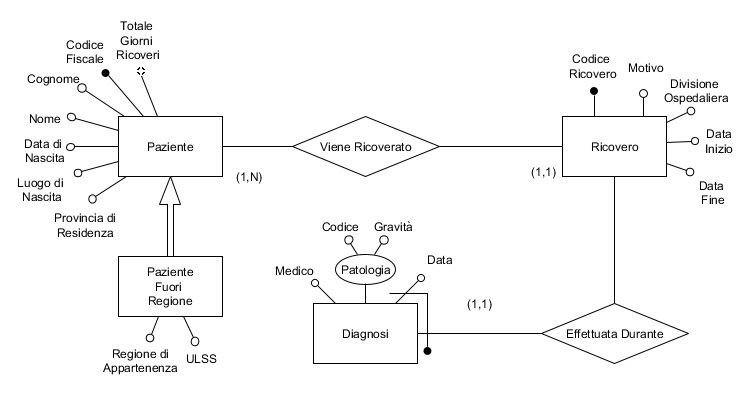
\includegraphics[width=\linewidth]{parte1}
  \caption{Prima parte}
	\label{fig:paz-ric-dia}
\end{figure}

La seconda fase considera il quarto, il quinto e parte del sesto punto dell'analisi dei requisiti, nei quali si chiede di tener traccia delle terapie e dei farmaci utilizzati.
Per questi ultimi è stata creata l'entità FARMACO con attributi: \textit{Dose Giornaliera Raccomandata}, \textit{Nome Commerciale}, \textit{Azienda Produttrice} e due attributi multivalore \textit{Nome Principi Attivi} e \textit{Quantità Principi Attivi}.
La chiave primaria è data dall'attributo \textit{Nome Commerciale} in quanto univoco.
Un farmaco deve contenere uno o più principi attivi.
\\
I requisiti richiedono che una terapia possa curare più patologie, di conseguenza una terapia deve rappresentare un metodo standard con cui affrontare varie patologie.
Quindi l'entità TERAPIA non può contenere informazioni come data di inizio, data di fine oppure medico prescrivente, altrimenti non sarebbe più generale.
Per questi motivi all'entità sono stati attribuiti i campi: \textit{Dose Giornaliera} e \textit{Modalità Somministrazione}.
Le richieste dei requisiti quali data di inizio e di fine e medico prescrivente della terapia verrano trattate nella terza fase di progettazione.
La chiave di TERAPIA è composta dagli attributi \textit{Dose Giornaliera} e \textit{Modalità Somministrazione} e dalla relazione SOMMINISTRATO\_DURANTE che lega FARMACO a TERAPIA.
Questa relazione è della forma Uno-a-Molti in quanto in ogni terapia si somministra un solo farmaco mentre un farmaco può essere somministrato in più terapie.
È importate considerare il fatto che una terapia non può esistere senza un farmaco da somministrare, quindi la partecipazione di TERAPIA alla relazione SOMMINISTRATO\_DURANTE è totale.
D'altro canto un farmaco può essere memorizzato nella base di dati pur non essendo associato ad una particolare terapia, quindi la partecipazione di FARMACO alla precedente relazione è parziale.
Il risultato della seconda fase di progettazione è illustrata nella \autoref{fig:far-ter}.

\begin{figure}[!ht] % TODO abbellire
  \centering
  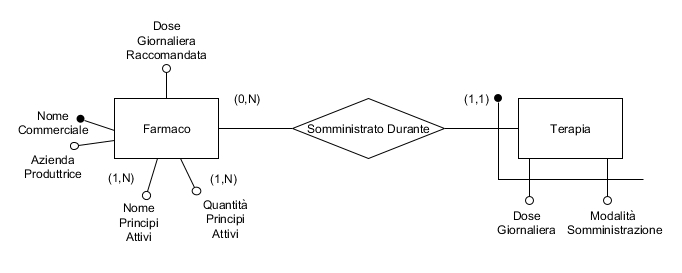
\includegraphics[width=\linewidth]{parte2}
  \caption{Seconda parte}
	\label{fig:far-ter}
\end{figure}

Nella terza fase della progettazione è stato modellato l'ultimo punto dell'analisi dei requisiti attraverso la relazione MOTIVA\_TERAPIA.
Particolare attenzione è stata fatta alla parte in cui si specifica che una terapia può essere associata ad una diagnosi in due modi differenti: quello che la definisce come cura per una patologia e quello che la definisce come causa di una nuova patologia.
Va sottolineato che in entrambi i casi, nella base di dati, la patologia è salvata attraverso DIAGNOSI.

In un primo momento è stato modellato il sottoschema illustrato in \autoref{fig:piccolo1}.
Il modo in cui è stata definita l'entità TERAPIA permette di modellare il requisito \textit{"ogni terapia può curare più patologie"}.
Un'informazione come data di inizio, o data di fine, o medico prescrivente, non può essere memorizzata in TERAPIA perché, altrimenti, non sarebbe possibile applicare questa stessa terapia in uno spazio temporale differente, pena la perdita delle informazioni precedenti.
D'altra parte non è nemmeno accettabile includere nella chiave primaria le informazioni relative alle date ed al medico, perché così facendo si differenzierebbero le entità, andando contro il requisito che si vuole modellare.
Da qui la necessità di omettere attributi data inizio, data fine e medico prescrivente in TERAPIA, assegnandoli alla relazione MOTIVA\_TERAPIA.
Intuitivamente questi attributi riguardano contemporaneamente la diagnosi, quindi la patologia che si vuole curare, e la terapia applicata, quindi il modo in cui si vuole affrontare la patologia, indicando il periodo in cui la terapia viene applicata e chi ha definito questo periodo.
Nei requisiti è specificato che per alcune patologie mancano le cure, per questo motivo la partecipazione a MOTIVA\_TERAPIA di DIAGNOSI è parziale.
Invece è sensato pensare che, se una terapia esiste, può curare almeno una patologia, quindi la partecipazione di TERAPIA alla relazione è totale.
Nel complesso MOTIVA\_TERAPIA, per ora, risulta essere una relazione Uno-A-Molti: nel testo è specificato che ad ogni diagnosi può essere associata al più una terapia.
Mentre TERAPIA è stata definita appositamente per poter esser associata a più DIAGNOSI. 

\begin{figure}[!ht] % TODO abbellire
  \centering 
  \begin{minipage}{.5\textwidth}
    \centering
    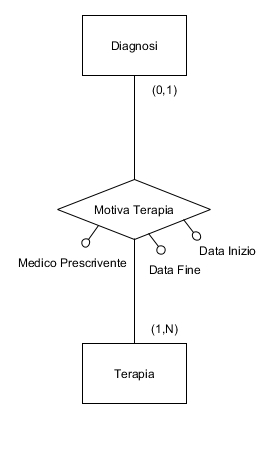
\includegraphics[width=\linewidth]{piccolo1}
    \caption{Prima modellazione}
    \label{fig:piccolo1}
  \end{minipage}%
  \begin{minipage}{.5\textwidth}
    \centering
    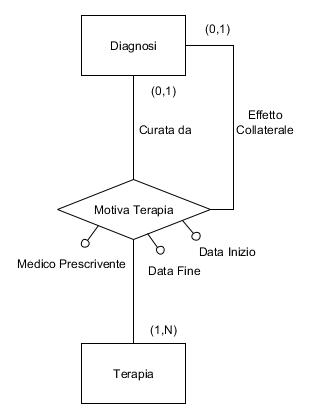
\includegraphics[width=\linewidth]{piccolo2}
    \caption{Relazione completa}
    \label{fig:piccolo2}
  \end{minipage}
\end{figure}

Successivamente è stato necessario modellare la situazione in cui una terapia prescritta è causa di una nuova patologia.  L'informazione che si vuole mantenere non dipende esclusivamente dall'entità TERAPIA ma dipende anche dal periodo di applicazione, quindi non è sufficiente creare una nuova relazione tra TERAPIA e DIAGNOSI, in quanto le informazioni aggiuntive sulla terapia sono memorizzate sulla relazione che le lega.  
La soluzione migliore è quella di trasformare MOTIVA\_TERAPIA in una relazione ternaria: con DIAGNOSI che partecipa da una parte come patologia in cura e dall'altra come rilevazione di una nuova patologia.  
Per comodità, il risultato di tale trasformazione è riportato in \autoref{fig:piccolo2}.  
Ricordando che non tutte le applicazioni di una terapia causano un effetto collaterale e che ne possono causare al massimo uno, la partecipazione di DIAGNOSI come effetto collaterale è parziale con cardinalità 1. 

Al termine di questa terza fase di progettazione è necessario introdurre dei vincoli d'integrità per la relazione ternaria:
\begin{itemize}
  \item in nessuna tripletta di MOTIVA\_TERAPIA può comparire due volte la stessa DIAGNOSI;
  \item le DIAGNOSI devono essere state effettuate durante lo stesso ricovero;
  \item la DIAGNOSI che partecipa come effetto collaterale deve avere una data successiva alla data della prima diagnosi, ma comunque precedente alla data di fine ricovero.
\end{itemize}
Nella fase logica verrà mostrato che questa relazione può essere trasformata, senza perdita d'informazione, con l'aggiunta di una nuova entità, in tre relazioni binarie. 

Nei requisiti è richiesto di memorizzare il medico che ha effettuato la diagnosi ed il medico che ha prescritto la terapia.
Ciò è stato fatto riportando rispettivamente le due informazioni nell'attributo \textit{Medico} in DIAGNOSI e nell'attributo \textit{Medico Prescrivente} in MOTIVA\_TERAPIA.
Non è stata introdotta un'entità MEDICO perché avrebbe contenuto soltanto l'informazione riguardante nome e cognome del medico.
Inoltre non è richiesto di tener traccia dello storico delle prescrizioni o delle diagnosi rispetto ai medici.
In conclusione lo schema Entità-Relazioni si presenta come in \autoref{fig:ER_progettazione_modello}.

\begin{figure}[H] % TODO abbellire
    \centering
    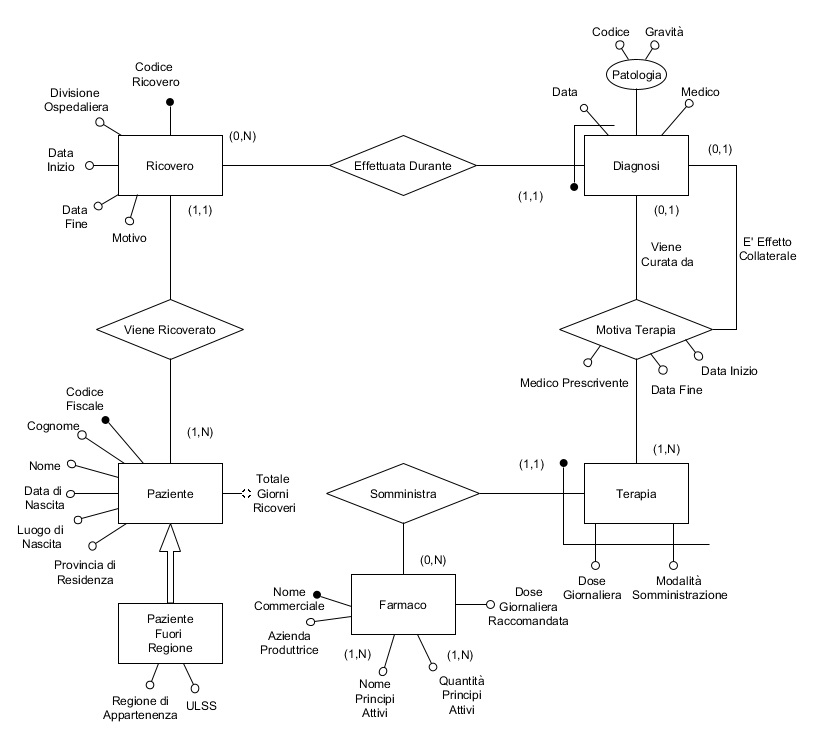
\includegraphics[width=\linewidth]{schema1}
    \caption{Lo schema Entità-Relazioni completo}
    \label{fig:ER_progettazione_modello}
\end{figure}




\clearpage
\section{Progettazione Logica}

\subsection{Ristrutturazione del Modello E-R}

È utile semplificare strutture come specializzazioni, attributi composti e attributi multivalore perché renderà più facile la traduzione del modello Entità-Relazioni in quello Relazionale.

\subsubsection{Semplificazione dei Concetti}

Il modello Relazione non permette di rappresentare generalizzazioni sarà necessario rimuovere tutte le specializzazioni dal nostro schema E-R.
Si può notare che la specializzazione PAZIENTE\_FUORI\_REGIONE può essere facilmente rappresentata aggiungendo due attributi all'entità PAZIENTE.
I nuovi attributi, \textit{ULSS} e \textit{Regione di Appartenenza}, in PAZIENTE saranno facoltativi poiché la specializzazione è parziale.
La rimozione delle generalizzazioni non è sempre così immediata: se PAZIENTE\_FUORI\_REGIONE avesse avuto una relazione aggiuntiva rispetto al genitore si sarebbero dovute valutare varie opzioni.
Per esempio la creazione di una nuova relazione tra genitore e figlio per mantenere il legame con gli attributi facoltativi.
Oppure la duplicazione nel figlio di tutti gli attributi e di tutte le relazioni del genitore.

Anche nel caso degli attributi composti la semplificazione è intuitiva, infatti nello schema l'unico attributo composto è \textit{Patologia} in DIAGNOSI.
L'attributo \textit{Patologia} può essere trasformato in due nuovi attributi \textit{Codice Patologia} e \textit{Gravità Patologia} contenenti esattamente la stessa informazione.



Bisogna prestare più attenzione agli attributi multivalore:
in FARMACO sono presenti \textit{Nome Principi Attivi} e \textit{Quantità Principi Attivi} entrambi obbligatori e multivalore.
L'unica semplificazione attuabile è creare una nuova entità chiamata PRINCIPIO\_ATTIVO e metterla in relazione Molti-A-Molti con FARMACO attraverso la nuova relazione CONTIENE.
Poiché i nomi dei principi attivi possono essere molto lunghi e non hanno un formato standard, in PRINCIPIO\_ATTIVO, sono salvati nella variabile \textit{Nome}, mentre una sequenza numerica chiamata \textit{Codice Principio Attivo} viene usata come chiave primaria.
Alla relazione CONTIENE è stato aggiunto l'attributo \textit{Quantità}.
In questo modo saranno modellate esattamente le stesse informazioni precedentemente modellate dagli attributi multivalore.
In realtà ora le informazioni sono salvate in un formato meno equivoco: prima non era chiaro come si mantenessero in relazione il nome del principio attivo e la sua quantità.

\begin{figure}[!ht] % TODO abbellire
  \centering
  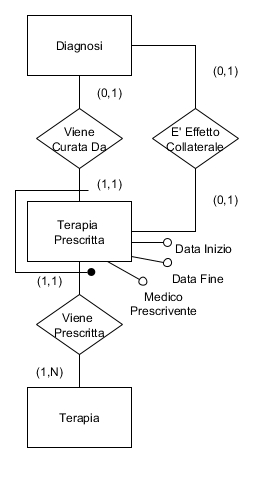
\includegraphics[width=.4\linewidth]{piccolo3}
  \caption{Il risultato della trasformazione di MOTIVA\_TERAPIA}
  \label{fig:piccolo3}
\end{figure}

Un'ulteriore trasformazione da effettuare riguarda la relazione ternaria.
Infatti MOTIVA\_TERAPIA, come è stato accennato in precedenza, può essere espressa tramite relazioni binarie.
In \autoref{fig:piccolo3} si può vedere il risultato di tale trasformazione.
Si nota subito la nuova entità TERAPIA\_PRESCRITTA, creata proprio per rappresentare una particolare applicazione di una terapia al fine di curare una patologia di una specifica diagnosi.
La nuova entità, quindi, è caratterizzata da:
\textit{Data Inizio} che indica il giorno in cui il paziente dovrà iniziare la terapia;
\textit{Data Fine} che indica il giorno in cui il paziente terminerà la terapia;
\textit{Medico Prescrivente} che indica il medico che ha prescritto la terapia e deciso il periodo di applicazione.
Osservando che la relazione MOTIVA\_TERAPIA non può esistere senza la partecipazione simultanea di DIAGNOSI (come \textit{Viene Curata da}) e di TERAPIA si è deciso di rendere TERAPIA\_PRESCRITTA un'entità debole.
La chiave primaria è composta dalle nuove relazioni binare VIENE\_CURATA\_DA e VIENE\_PRESCRITTA, per entrambe la partecipazione di TERAPIA\_PRESCRITTA è totale, mentre la cardinalità è al massimo uno.
DIAGNOSI e TERAPIA interagiscono con le nuove relazioni, rispettivamente, nello stesso modo con cui interagivano con la relazione ternaria.
Per quanto riguarda È\_EFFETTO\_COLLATERALE si può dire che cattura la possibilità che una terapia prescritta possa causare una nuova patologia.
Notare che le partecipazioni sono appunto parziali.
Bisognerà modificare oppure aggiungere alcuni vincoli d'integrità:
\begin{itemize}
  \item TERAPIA\_PRESCRITTA non può essere in relazione È\_EFFETTO\_COL-LATERALE con la DIAGNOSI con cui definisce la sua chiave primaria;
  \item TERAPIA\_PRESCRITTA non può essere in relazione È\_EFFETTO\_COL-LATERALE con una DIAGNOSI avente una data che precede la data della DIAGNOSI con cui definisce la sua chiave primaria;
  \item la data d'inizio della TERAPIA\_PRESCRITTA deve essere compresa tra la data della DIAGNOSI che la definisce e la data della DIAGNOSI che identifica l'effetto collaterale;
  \item la data di fine della TERAPIA\_PRESCRITTA non può precedere la sua data di inizio.
\end{itemize}
A questo punto, osservando nuovamente i sottoschemi in \autoref{fig:piccolo2} ed in \autoref{fig:piccolo3}, è chiaro che modellino ogni possibile situazione:
\begin{itemize}
  \item una DIAGNOSI a cui non è ancora stata assegnata una terapia;
  \item la prescrizione di una specifica terapia;
  \item la scoperta di una nuova patologia (attraverso una nuova diagnosi) causata dall'applicazione di una terapia;
  \item la possibilità che una TERAPIA possa curare più patologie (registrate attraverso DIAGNOSI differenti).
%TODO ci sono tutte?
\end{itemize}

Durante la fase di semplificazione dei concetti vengono analizzate anche le chiavi primarie delle entità.
Quando una chiave è troppo complessa, cioè composta da molti elementi, è bene sostituirla, così facendo si faciliteranno tutte le operazioni sulla base di dati.
Si ricorda che un'entità può disporre di chiavi candidate, cioè insiemi di attributi che, per loro natura, rispettano la proprietà di chiave primaria ma che, per qualche motivo, non sono stati scelti come tale.
Ora è naturale verificare se tra queste chiavi opzionali ce n'è una che, dopo tutte le semplificazioni effettuate allo schema E-R, è migliore della chiave primaria.
Purtroppo questa strada non è sempre percorribile, infatti non è raro che le entità siano tra loro distinguibili soltanto per mezzo di un preciso insieme di attributi.
Nello schema E-R considerato fino ad ora non sono presenti chiavi candidate migliori delle chiavi primarie attuali, infatti la chiave primaria della maggior parte delle entità è composta da un solo attributo.

Rimangono da analizzare DIAGNOSI, TERAPIA e la nuova\\TERAPIA\_PRESCRITTA.
La chiave primaria di quest'ultima, per il modo in cui l'entità è stata costruita, non può essere modificata a meno di introdurre pesanti vincoli di integrità.
Ora sorge un problema: TERAPIA\_PRESCRITTA è un'entità debole che dipende da due entità a loro volta deboli.
Ciò significa che per identificare una terapia prescritta si deve risalire al ricovero da una parte ed al farmaco dall'altra, nel mentre si deve anche ricordare \textit{Data} in DIAGNOSI e \textit{Dose Giornaliera} e \textit{Modalità Somministrazione} in TERAPIA.
Intuitivamente questo equivale ad avere una chiave primaria in TERAPIA\_PRESCRITTA composta da 5 elementi.
Quindi si propone di creare sia in DIAGNOSI che in TERAPIA un nuovo attributo chiamato, rispettivamente, \textit{Codice Diagnosi} e \textit{Codice Terapia} che conterrà un valore numerico simile a quello contenuto in \textit{Codice Ricovero}.

Applicando tutte le semplificazioni sopra descritte si ottiene lo schema E-R illustrato In \autoref{fig:ER_ristrutturato}.

\begin{figure}[H] % TODO abbellire
	\centering
	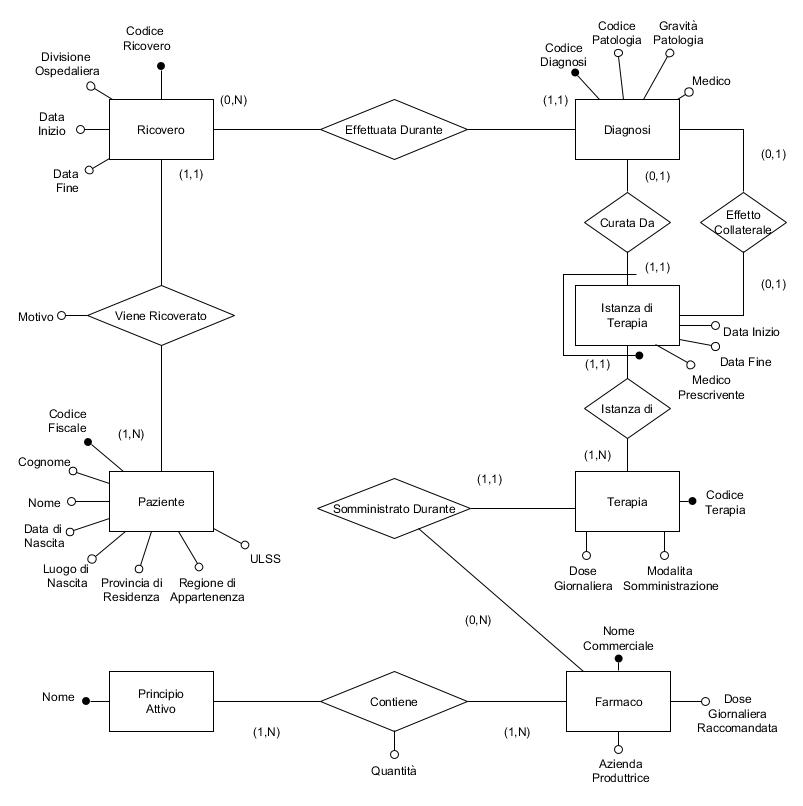
\includegraphics[width=\linewidth]{schema2}
	\caption{Lo schema Entità-Relazioni ristrutturato}
  \label{fig:ER_ristrutturato}
\end{figure}




\clearpage
\subsubsection{Analisi delle Ridondanze}

Gli attributi derivati, come può suggerire il nome, conservano dati già presenti nella base di dati, quindi introducono ridondanza.
Si ricorda che quest'ultima, quando si progetta una base di dati, è da evitare, non tanto perché l'informazione ripetuta occupa spazio doppio, ma piuttosto perché si rischia di introdurre pericolose inconsistenze.
Detto ciò, gli attributi derivati sono utili se mantengono informazione che altrimenti sarebbe dispendioso ottenere, oppure informazione richiesta molto spesso.
In entrambi i casi un attributo derivato velocizza il recupero del dato, introducendo però del carico aggiuntivo in fase di inserimento od aggiornamento dello stesso.

Sfruttando i volumi stimati durante l'analisi dei requisiti si valuterà se conviene o meno mantenere l'attributo derivato \textit{Totale Giorni Ricoveri} dell'entità PAZIENTE.
In \autoref{fig:attributo-ridondante} è stata riportata una sezione dello schema relazionale.
\begin{figure}[H] % TODO abbellire
	\centering
	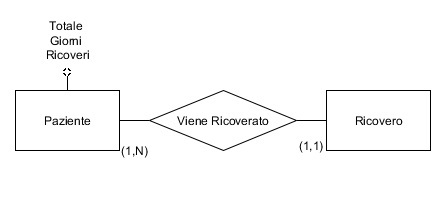
\includegraphics[width=\linewidth]{totalegiorni}
	\caption{Attributo derivato Totale Giorni Ricoveri}
	\label{fig:attributo-ridondante}
\end{figure}

I volumi stimati sono riportati in \autoref{tab:volumi-attributo-ridondante} e la frequenza delle operazioni interessate in \autoref{tab:operazioni-attributo-ridondante}.

\begin{table}[H]
	\centering
	\begin{tabular}{|l|c|r|}
		\hline
		\textbf{Concept} & \textbf{Type} & \textbf{Volume} \\ \hline
		Paziente         & E             & 100000          \\ \hline
		Ricovero         & E             & 300000          \\ \hline
		Viene Ricoverato & R             & 300000          \\ \hline
	\end{tabular}
	\caption{Tabella dei volumi ridotta}
	\label{tab:volumi-attributo-ridondante}
\end{table}

\begin{table}[H]
	\centering
	\begin{tabular}{|l|c|r|}
		\hline
		\textbf{Operation}                  & \textbf{Type} & \textbf{Frequency} \\ \hline
		Registrazione Ricovero              & I             & 175/giorno         \\ \hline
		Controllo totale giorni di ricoveri & I             & 175/giorno         \\ \hline %TODO fix questo numero
	\end{tabular}
	\caption{Tabella delle operazioni ridotta}
	\label{tab:operazioni-attributo-ridondante}
\end{table}

In presenza dell'attributo derivato, per l'operazione di registrazione di un nuovo ricovero è necessario 1 accesso in scrittura per l'entità RICOVERO, 1 accesso in scrittura per la relazione VIENE\_RICOVERATO, 1 accesso in lettura ed 1 accesso in scrittura per l'entità PAZIENTE per leggere e aggiornare l'attributo \textit{Totale Giorni Ricoveri}.
Per l'operazione di verifica del totale dei giorni di ricoveri è sufficiente 1 accesso in lettura all'entità PAZIENTE.

\cleardoublepage

\begin{table}[H]
	\centering
	\begin{tabular}{|l|c|c|c|}
		\hline
		\textbf{Concept} & \textbf{Type} & \textbf{Access} & \textbf{Type} \\ \hline
		\multicolumn{4}{|c|}{Registrazione Ricovero}                       \\ \hline
		Ricovero         & E             & 1               & W             \\ \hline
		Viene Ricoverato & R             & 1               & W             \\ \hline
		Paziente         & E             & 1               & R             \\ \hline
		Paziente         & E             & 1               & W             \\ \hline
		\multicolumn{4}{|c|}{Controllo totale giorni di ricoveri}          \\ \hline
		Paziente         & E             & 1               & R             \\ \hline
	\end{tabular}
	\caption{Tabella dei costi, caso con ridondanza}
	\label{tab:costi-attributo-ridondante}
\end{table}


Considerando il costo di 1 accesso in scrittura come 2 accessi in lettura, si calcola il numero di accessi complessivo giornaliero per le 2 operazioni nel caso con ridondanza:
\begin{equation}
	(3W + 1R) \times 175 + 1R \times 175 \approx 1400R
\end{equation}

Rimuovendo l'attributo, per l'operazione di registrazione di un nuovo ricovero è sufficiente 1 accesso in scrittura per l'entità RICOVERO e 1 accesso in scrittura per la relazione VIENE\_RICOVERATO.
Per l'operazione di verifica del totale dei giorni di ricoveri, considerando la tabella dei volumi, sono necessari in media 3 accessi in lettura per la relazione VIENE\_RICOVERATO e 3 accessi in lettura per l'entità RICOVERO.

\begin{table}[H]
	\centering
	\begin{tabular}{|l|c|c|c|}
		\hline
		\textbf{Concept} & \textbf{Type} & \textbf{Access} & \textbf{Type} \\ \hline
		\multicolumn{4}{|c|}{Inserimento Diagnosi}                         \\ \hline
		Viene Ricoverato & R             & 1               & W             \\ \hline
		Ricovero         & R             & 1               & W             \\ \hline
		\multicolumn{4}{|c|}{Stampa Storico Diagnosi}                      \\ \hline
		Viene Ricoverato & R             & 3               & R             \\ \hline
		Ricovero         & E             & 3               & R             \\ \hline
	\end{tabular}
	\caption{Tabella dei costi, caso senza ridondanza}
	\label{tab:costi-no-attributo-ridondante}
\end{table}

Considerando il costo di 1 accesso in scrittura come 2 accessi in lettura, si calcola il numero di accessi complessivo giornaliero per le 2 operazioni nel caso senza ridondanza:
\begin{equation}
	2W \times 175 + 6R \times 175 \approx 1750R
\end{equation}

Risulta conveniente mantenere l'attributo \textit{Totale Giorni Ricoveri}.

Lo schema Entità-Relazioni in \autoref{fig:ER_ristrutturato} non presenta ulteriori ridondanze.
Il ciclo formato dalle entità DIAGNOSI, TERAPIA\_PRESCRITTA e DIAGNOSI non crea ridondanze perché ogni elemento fornisce un'informazione unica: la prima diagnosi giustifica la cura, la terapia prescritta spiega quando tale cura è stata applicata, mentre la seconda diagnosi riporta eventuali effetti collaterali.

Nei requisiti è specificato che l'ospedale visualizza molto spesso le diagnosi dei pazienti, senza richiedere necessariamente i dati relativi ai ricoveri.
Per questo motivo si è considerata la possibilità di aggiungere una nuova relazione:
\begin{itemize}
	\item EFFETTUATA\_A: una relazione Uno-A-Molti tra PAZIENTE e DIAGNOSI.
    La partecipazione di PAZIENTE è parziale mentre quella di DIAGNOSI è totale.
\end{itemize}

Viene creato quindi il ciclo in \autoref{fig:ciclo-ridondanza} PAZIENTE, RICOVERO, DIAGNOSI dato dalle relazioni VIENE\_RICOVERATO, EFFETTUATA\_DURANTE, EFFETTUATA\_A.

\begin{figure}[H] % TODO abbellire
	\centering
	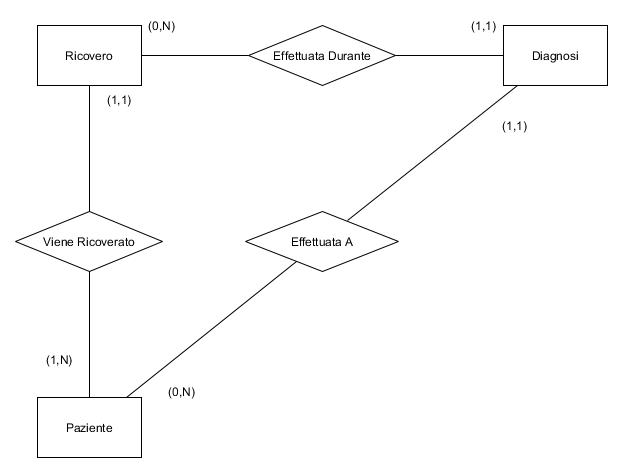
\includegraphics[width=\linewidth]{schema3}
	\caption{Ciclo con ridondanza}
	\label{fig:ciclo-ridondanza}
\end{figure}

%TODO latex non sa dividere le parole tipo parola-parola
Si procede con il valutare se è conveniente mantenere la relazione EFFET-
TUATA\_A tra PAZIENTE e DIAGNOSI in funzione della frequenza delle operazioni di inserimento nuove diagnosi e stampa dello storico diagnosi di un paziente.

% TODO REQUISITO specificare nei requisiti le operazioni richieste e i volumi
% TODO per questione estetica spostare una tabella o del testo qua, cosi' non rimane un buco a fine pagina

I volumi stimati sono riportati in \autoref{tab:volumi-ciclo} e la frequenza delle operazioni interessate in \autoref{tab:operazioni-ciclo}

% TODO REQUISITO spostare table:volumi nei requisiti, no non si può non tutti esistono nei requisiti
\begin{table}[H]
	\centering
	\begin{tabular}{|l|c|r|}
		\hline
		\textbf{Concept}      & \textbf{Type} & \textbf{Volume} \\ \hline
		Paziente              & E             & 100000          \\ \hline
		Ricovero              & E             & 300000          \\ \hline
		Diagnosi              & E             & 1200000         \\ \hline
		Terapia               & E             & 30000           \\ \hline
		Istanza di Terapia    & E             & 1100000         \\ \hline
		Farmaco               & E             & 10000           \\ \hline
		Viene Ricoverato      & R             & 300000          \\ \hline
		Effettuata Durante    & R             & 1200000         \\ \hline
		Effettuta A           & R             & 1200000         \\ \hline
		Curata Da             & R             & 1100000         \\ \hline
		Istanza Di            & R             & 1100000         \\ \hline
		Effetto Collaterale   & R             & 50000           \\ \hline
		Somministrato Durante & R             & 10000           \\ \hline
	\end{tabular}
	\caption{Tabella dei volumi}
	\label{tab:volumi}
\end{table}

\begin{table}[H]
	\centering
	\begin{tabular}{|l|c|r|}
		\hline
		\textbf{Concept}   & \textbf{Type} & \textbf{Volume} \\ \hline
		Paziente           & E             & 100000          \\ \hline
		Ricovero           & E             & 300000          \\ \hline
		Diagnosi           & E             & 1200000         \\ \hline
		Viene Ricoverato   & R             & 300000          \\ \hline
		Effettuata Durante & R             & 1200000         \\ \hline
		Effettuata A       & R             & 1200000         \\ \hline
	\end{tabular}
	\caption{Tabella dei volumi ridotta}
	\label{tab:volumi-ciclo}
\end{table}

\begin{table}[H]
	\centering
	\begin{tabular}{|l|c|r|}
		\hline
		\textbf{Operation}      & \textbf{Type} & \textbf{Frequency} \\ \hline
		Inserimento Diagnosi    & I             & 700/giorno         \\ \hline
		Stampa Storico Diagnosi & I             & 1400/giorno        \\ \hline
	\end{tabular}
	\caption{Tabella delle operazioni ridotta}
	\label{tab:operazioni-ciclo}
\end{table}

Nel caso con ridondanza per l'operazione di inserimento di una nuova diagnosi sono necessari 1 accesso in scrittura per l'entità DIAGNOSI e 1 accesso in scrittura per entrambe le relazioni EFFETTUATA\_DURANTE e EFFETTUATA\_A.
Per l'operazione di stampa delle diagnosi di un paziente sono necessari 12 accessi in lettura per la relazione EFFETTUATA\_A e 12 accessi in lettura per l'entità DIAGNOSI.

Considerando il costo di 1 accesso in scrittura come 2 accessi in lettura, si calcola il numero di accessi complessivo giornaliero per le 2 operazioni nel caso con ridondanza:
\begin{equation}
	3W \times 700 + 24R \times 1400 \approx	37800R
\end{equation}

\begin{table}[H]
	\label{table:3}
	\centering
	\begin{tabular}{|l|c|c|c|}
		\hline
		\textbf{Concept}    & \textbf{Type} & \textbf{Access} & \textbf{Type} \\ \hline
		\multicolumn{4}{|c|}{Inserimento Diagnosi}                            \\ \hline
		Diagnosi            & E             & 1               & W             \\ \hline
		Effettutata Durante & R             & 1               & W             \\ \hline
		Effettuata A        & R             & 1               & W             \\ \hline
		\multicolumn{4}{|c|}{Stampa Storico Diagnosi}                         \\ \hline
		Effettuata A        & R             & 12              & R             \\ \hline
		Diagnosi            & E             & 12              & R             \\ \hline
	\end{tabular}
	\caption{Tabella dei costi, caso con ridondanza}
\end{table}

Nel caso senza ridondanza per l'operazione di inserimento di una nuova diagnosi sono necessari 1 accesso in scrittura per l'entità DIAGNOSI e 1 accesso in scrittura per la relazione EFFETTUATA\_DURANTE.
Per l'operazione di stampa delle diagnosi di un paziente sono necessari 3 accessi in lettura per la relazione VIENE\_RICOVERATO, 12 accessi in lettura per la relazione EFFETTUATA\_DURANTE e 12 accessi in lettura per l'entità DIAGNOSI.

Considerando il costo di 1 accesso in scrittura come 2 accessi in lettura, si calcola il numero di accessi complessivo giornaliero per le 2 operazioni nel caso senza ridondanza:
\begin{equation}
	2W \times 700 + 27R \times 1400 \approx	40600R
\end{equation}

\begin{table}[H]
	\label{table:4}
	\centering
	\begin{tabular}{|l|c|c|c|}
		\hline
		\textbf{Concept}    & \textbf{Type} & \textbf{Access} & \textbf{Type} \\ \hline
		\multicolumn{4}{|c|}{Inserimento Diagnosi}                            \\ \hline
		Diagnosi            & E             & 1               & W             \\ \hline
		Effettutata Durante & R             & 1               & W             \\ \hline
		\multicolumn{4}{|c|}{Stampa Storico Diagnosi}                         \\ \hline
		Viene Ricoverato    & R             & 3               & R             \\ \hline
		Effettutata Durante & R             & 12              & R             \\ \hline
		Diagnosi            & E             & 12              & R             \\ \hline
	\end{tabular}
	\caption{Tabella dei costi, caso senza ridondanza}
\end{table}

Concludiamo che è conveniente mantenere la ridondanza visto il costo minore delle operazioni giornaliere.

\begin{figure}[!ht] % TODO abbellire
    \centering
    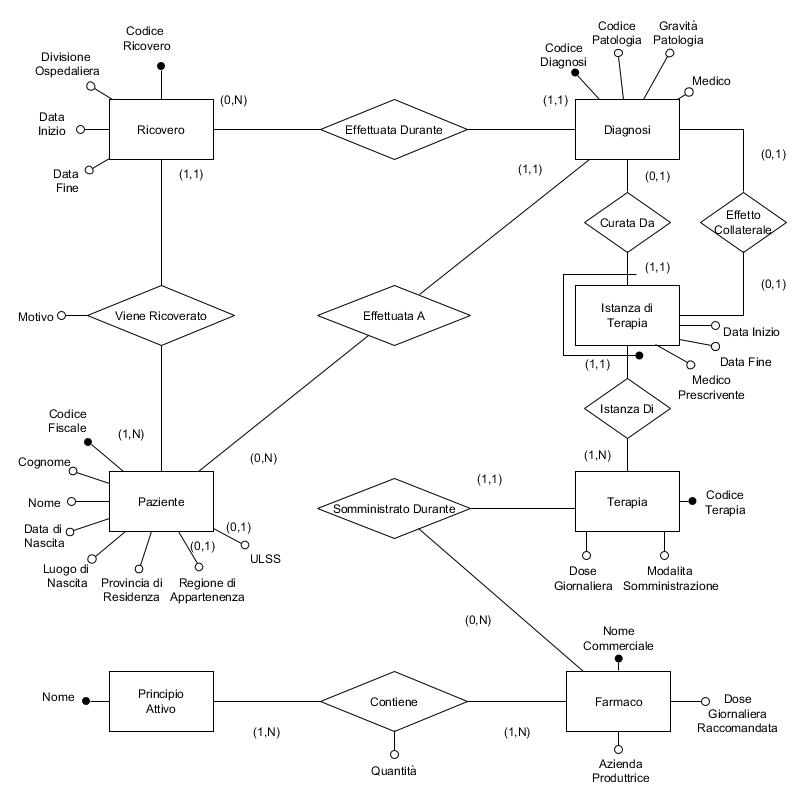
\includegraphics[width=\linewidth]{schema4}
    \caption{Lo schema Entità-Relazioni finale}
    \label{fig:ER_finale}
\end{figure}



\clearpage
\subsection{Traduzione da ER a Relazionale}


% TODO leggere capitolo 14 Elmasri
% TODO leggere capitolo 9 Atzeni

In questa fase della progettazione logica è possibile iniziare la traduzione del modello E-R in quello Relazionale.
Come prima cosa, in quanto immediato, ogni entità verrà rappresentata sotto forma di tupla.
Queste tuple verranno poi modificate per poter mantenere anche le informazioni relative alle relazioni, può capitare che ad una relazione venga associata un nuova tupla.

In \autoref{fig:relazionale_iniziale} si può vedere una prima modellazione dello schema Relazionale, con le seguenti tuple:
\begin{itemize}
  \item PAZIENTE(\textit{\underline{cf}, cognome, nome, data\_nasc, luogo\_nasc, prov\_res, reg\_app, ulss, tot\_gg\_ric}) con \textit{cf} come chiave primaria.
  \item RICOVERO(\textit{\underline{cod\_ric}, data\_i, data\_f, motivo, div\_osp}) con \textit{cod\_ric} come chiave primaria;
  \item DIAGNOSI(\textit{\underline{cod\_dia}, data\_dia, cod\_pat, medico}) con \textit{cod\_dia} come chiave primaria;
  \item TERAPIA(\textit{\underline{cod\_ter}, dose\_gio, mod\_somm, farmaco}) con \textit{cod\_ter} come chiave primaria;
  \item FARMACO(\textit{\underline{nome\_comm}, azienda\_prod, dose\_gg\_racc}) con \textit{nome\_comm}\\come chiave primaria;
  \item PRINCIPIO\_ATTIVO(\textit{\underline{cod\_pa}}, \textit{nome}) con \textit{cod\_pa} come chiave primaria.
\end{itemize}
Bisogna prestare più attenzione a TERAPIA\_PRESCRITTA perché, in quanto entità debole, la sua chiave primaria dipende dalle relazioni\\VIENE\_CURATA\_DA e VIENE\_PRESCRITTA, o meglio, comprende degli\\identificatori esterni.
Nel dettaglio un identificatore sarà dato dalla chiave primaria di DIAGNOSI mentre l'altro dalla chiave primaria di TERAPIA.
Si ricorda che le entità identificate esternamente partecipano alle associazioni identificanti sempre con una cardinalità minima e massima pari a uno.
Quindi, nonostante le due relazioni siano di tipi differenti (Uno-A-Uno ed Uno-A-Molti), possono essere trattate allo stesso modo, cioè aggiungendo alla tupla
\vspace{3mm}
\\
\hspace{10mm}
TERAPIA\_PRESCRITTA(\textit{data\_i, data\_f, med\_presc})
\vspace{3mm}
\\
i nuovi valori referenziali \textit{diagnosi} e \textit{terapia}.
Questi, rispettivamente, conterranno il valore \textit{cod\_dia} e \textit{cod\_ter} delle tuple dalle quali TERAPIA\_PRESCRITTA dipende.
La tupla risultante è la seguente:
\vspace{3mm}
\\ TERAPIA\_PRESCRITTA(\textit{\underline{diagnosi}, \underline{terapia}, data\_i, data\_f, med\_presc})
\vspace{3mm}
\\
la chiave primaria è composta dalla coppia (\textit{diagnosi, terapia}).


\begin{figure}
\begin{tikzpicture}
  [relation/.style={
    rectangle split,
    rectangle split parts=#1,
    rectangle split part align=base,
    draw,
    anchor=center,
    align=center,
    text height=3mm,
    text centered
    }
  ]
  \hspace*{-0.6cm} % tutto un po' più a  sinistra
  
  \node (pazientetitle) {\textbf{PAZIENTE}};
  \node [
    relation=9,
    rectangle split horizontal,
    rectangle split part fill={lightgray!50},
    anchor=north west,
    below=0.6cm of pazientetitle.west,
    anchor=west
    ]
    (paziente)
    {
     \nodepart{one}    \underline{cf}
     \nodepart{two}    cognome
     \nodepart{three}  nome
     \nodepart{four}   data\_nasc
     \nodepart{five}   luogo\_nasc
     \nodepart{six}    prov\_res
     \nodepart{seven}  reg\_app
     \nodepart{eight}  ulss
     \nodepart{nine}   tot\_gg\_ric
    };
  
  \node [below=1.3cm of paziente.west, anchor=west] (ricoverotitle) {\textbf{RICOVERO}};
  \node [
    relation=5,
    rectangle split horizontal,
    rectangle split part fill={lightgray!50},
    anchor=north west,
    below=0.6cm of ricoverotitle.west,
    anchor=west
    ]
    (ricovero)
    {
     \nodepart{one}  \underline{cod\_ric}
     \nodepart{two}   data\_i
     \nodepart{three} data\_f
     \nodepart{four}  motivo
     \nodepart{five}  div\_osp
    };
  
  \node [below=1.3cm of ricovero.west, anchor=west] (diagnosititle) {\textbf{DIAGNOSI}};
  \node [
    relation=5,
    rectangle split horizontal,
    rectangle split part fill={lightgray!50},
    anchor=north west,
    below=0.6cm of diagnosititle.west,
    anchor=west
    ]
    (diagnosi)
    {
     \nodepart{one} \underline{cod\_dia}
     \nodepart{two}   data\_dia
     \nodepart{three} cod\_pat
     \nodepart{four}  grav\_pat
     \nodepart{five}  medico
    };
  
  \node [below=1.3cm of diagnosi.west, anchor=west] (terapiatitle) {\textbf{TERAPIA}};
   \node [
    relation=3,
    rectangle split horizontal,
    rectangle split part fill={lightgray!50},
    anchor=north west,
    below=0.6cm of terapiatitle.west,
    anchor=west
    ]
    (terapia)
    {
      \nodepart{one}  \underline{cod\_ter}
     \nodepart{two}   dose\_gio
     \nodepart{three} mod\_somm
    };
  
  \node [below=1.3cm of terapia.west, anchor=west] (terapiaprescrittatitle) {\textbf{TERAPIA\_PRESCRITTA}};
  \node [
    relation=5,
    rectangle split horizontal,
    rectangle split part fill={lightgray!50},
    anchor=north west,
    below=0.6cm of terapiaprescrittatitle.west,
    anchor=west
    ]
    (terapiaprescritta)
    {
     \nodepart{one}   \underline{diagnosi}
     \nodepart{two}   \underline{terapia}
     \nodepart{three} data\_i
     \nodepart{four}  data\_f
     \nodepart{five}  med\_presc
    };
  
  \node [below=1.3cm of terapiaprescritta.west, anchor=west] (farmacotitle) {\textbf{FARMACO}};
  \node [
    relation=3,
    rectangle split horizontal,
    rectangle split part fill={lightgray!50},
    anchor=north west,
    below=0.6cm of farmacotitle.west,
    anchor=west
    ]
    (farmaco)
    {
     \nodepart{one}  \underline{nome\_comm}
     \nodepart{two}   dose\_gg\_racc
     \nodepart{three} azienda\_prod
    };
  
  \node [below=1.3cm of farmaco.west, anchor=west] (principiotitle) {\textbf{PRINCIPIO\_ATTIVO}};
  \node [
    relation=2,
    rectangle split horizontal,
    rectangle split part fill={lightgray!50},
    anchor=north west,
    below=0.6cm of principiotitle.west,
    anchor=west
    ]
    (principio)
    {
     \nodepart{one} \underline{cod\_pa}
     \nodepart{two} nome
    };

  \draw[-latex] (terapiaprescritta.one south) -- ++(0,-0.4) -| ($(terapiaprescritta.one south) + (7,0)$) |- ($(diagnosi.one south) + (-0,-0.6)$) -| ($(diagnosi.one south) + (-0,0)$);

  \draw[-latex] (terapiaprescritta.two south) -- ++(0,-0.2) -| ($(terapiaprescritta.two south) + (5.3,0)$) |- ($(terapia.one south) + (0,-0.6)$) -| ($(terapia.one south) + (0,0)$);
\end{tikzpicture}
\caption{Primo modello relazionale}
\label{fig:relazionale_iniziale}
\end{figure}


In questi passaggi, in realtà, è stato fatto qualcosa di più di una semplice traduzione di una entità dal modello E-R a quello Relazione, infatti sono state tradotte anche due relazioni.

La prima è VIENE\_CURATA\_DA che fornisce l'informazione: una patologia, trovata per mezzo di una diagnosi, può essere curata con l'applicazione di una particolare terapia.
Quest'informazione, nel modello relazionale, può essere trovata cercando, tra tutte le tuple per le terapie prescritte, una che abbia il campo \textit{diagnosi} uguale al campo \textit{cod\_dia} della DIAGNOSI.
Notare che non esiste nessuna certezza che tale tupla esista.
Questa possibilità è consistente con quanto modellato nello schema E-R (la partecipazione di DIAGNOSI è parziale).
Bisogna, invece, introdurre un vincolo che vieti che due tuple del tipo TERAPIA\_PRESCRITTA referenzino la stessa diagnosi, in altre parole bisogna assicurare la proprietà di chiave al campo \textit{diagnosi}.

La seconda relazione è VIENE\_PRESCRITTA.
Anche in questo caso il campo \textit{Terapia} permette di trovare tutte le particolari applicazioni di una data terapia.
In questo caso, poiché la relazione è del tipo Uno-A-Molti, la possibilità che lo stesso \textit{Codice\_Terapia} venga referenziato da tuple differenti non è un problema.
Invece, deve essere introdotto un vincolo d'integrità per assicurare che ogni TERAPIA salvata sia stata applicata almeno una volta (partecipazione totale).

Ora che tutte le entità sono state tradotte si può procedere alla traduzione delle relazioni.
Il risultato finale è rappresentato in \autoref{fig:relazionale_finale}.

VIENE\_RICOVERATO è del tipo Uno-A-Molti con entrambe le partecipazioni totali.
Come visto in precedenza non c'è modo di assicurare la partecipazione se non con dei vincoli esterni, in questo caso da applicare su RICOVERO.
La tupla che rappresenta i ricoveri deve essere modificata aggiungendo un campo per una chiave esterna chiamata \textit{Paziente}.

Anche le relazioni EFFETTUATA\_DURANTE, EFFETTUATA\_A e SOMMINISTRATA devono essere affrontate allo stesso modo, tutte del tipo Uno-A-Molti.
DIAGNOSI partecipa alle prime due con cardinalità pari a uno bisognerà quindi aggiungere due nuovi campi: il primo punterà alla chiave primaria di RICOVERO, mentre il secondo a quella di PAZIENTE.
Poiché una diagnosi deve essere necessariamente collegata ad un ricovero, dunque anche ad un paziente, i campi appena introdotti non possono essere lasciati vuoti.
A TERAPIA verrà aggiunta una chiave esterna contenente l'identificatore di FARMACO, anch'essa deve obbligatoriamente contenere un valore.

È\_EFFETTO\_COLLATERALE si differenzia dai casi precedenti non solo perché è del tipo Uno-A-Uno ma soprattutto perché non necessita di vincoli esterni, in quanto le due entità partecipano in modo parziale.
Data la simmetria della relazione, si può scegliere se modificare la tupla relativa a DIAGNOSI o quella di TERAPIA\_PRESCRITTA.
\\
Si è preferito usare quest'ultima perché le terapie prescritte sono in numero minore e ciò significa che ci saranno meno campi vuoti nella base di dati.

L'ultima relazione da analizzare è CONTIENE, del tipo Molti-A-Molti.
L'unico modo per trasformare questa relazione è creare una nuova tupla, che è stata chiamata CONTIENE ed è composta da tre valori: le chiavi esterne \textit{Farmaco} e \textit{Principio\_Attivo} seguite da \textit{Quantità}.
La chiave primaria della tupla è formata dai primi due valori in modo che un qualsiasi FARMACO possa essere messo in relazione con tutti i principi attivi necessari e, viceversa, che un PRINCIPIO\_ATTIVO possa essere contenuto in più farmaci.
Notare che è obbligatoria l'introduzione di due vincoli d'integrità, uno deve assicurare che un PRINCIPIO\_ATTIVO compaia in almeno un farmaco, l'altro che un farmaco contenga almeno un PRINCIPIO\_ATTIVO.

\begin{figure}
\begin{tikzpicture} % TODO abbellire
  [relation/.style={
    rectangle split,
    rectangle split parts=#1,
    rectangle split part align=base,
    draw,
    anchor=center,
    align=center,
    text height=3mm,
    text centered
    }
  ]
  \hspace*{-0.6cm} % tutto un po' più a  sinistra
  
  \node (pazientetitle) {\textbf{PAZIENTE}};
  \node [
    relation=9,
    rectangle split horizontal,
    rectangle split part fill={lightgray!50},
    anchor=north west,
    below=0.6cm of pazientetitle.west,
    anchor=west
    ]
    (paziente)
    {
     \nodepart{one}    \underline{cf}
     \nodepart{two}    cognome
     \nodepart{three}  nome
     \nodepart{four}   data\_nasc
     \nodepart{five}   luogo\_nasc
     \nodepart{six}    prov\_res
     \nodepart{seven}  reg\_app
     \nodepart{eight}  ulss
     \nodepart{nine}   tot\_gg\_ric
    };
  
  \node [below=1.3cm of paziente.west, anchor=west] (ricoverotitle) {\textbf{RICOVERO}};
  \node [
    relation=6,
    rectangle split horizontal, rectangle split part fill={lightgray!50},
    anchor=north west,
    below=0.6cm of ricoverotitle.west,
    anchor=west
    ]
    (ricovero)
    {
     \nodepart{one}  \underline{cod\_ric}
     \nodepart{two}   data\_i
     \nodepart{three} data\_f
     \nodepart{four}  motivo
     \nodepart{five}  div\_osp
     \nodepart{six}   paziente
    };
  
  \node [below=1.3cm of ricovero.west, anchor=west] (diagnosititle) {\textbf{DIAGNOSI}};
  \node [
    relation=7,
    rectangle split horizontal,
    rectangle split part fill={lightgray!50},
    anchor=north west,
    below=0.6cm of diagnosititle.west,
    anchor=west
    ]
    (diagnosi)
    {
     \nodepart{one}   \underline{cod\_dia}
     \nodepart{two}   data\_dia
     \nodepart{three} cod\_pat 
     \nodepart{four}  grav\_pat
     \nodepart{five}  medico
     \nodepart{six}   paziente
     \nodepart{seven} ricovero
    };
  
  \node [below=1.5cm of diagnosi.west, anchor=west] (terapiaprescrittatitle) {\textbf{TERAPIA\_PRESCRITTA}};
  \node [
    relation=6,
    rectangle split horizontal,
    rectangle split part fill={lightgray!50},
    anchor=north west,
    below=0.6cm of terapiaprescrittatitle.west,
    anchor=west
    ]
    (terapiaprescritta)
    {
     \nodepart{one}   \underline{terapia}
     \nodepart{two}   \underline{diagnosi}
     \nodepart{three} data\_i
     \nodepart{four}  data\_f
     \nodepart{five}  med\_presc
     \nodepart{six}   coll\_dia
    };
  
  \node [below=1.3cm of terapiaprescritta.west, anchor=west] (terapiatitle) {\textbf{TERAPIA}};
  \node [
    relation=4,
    rectangle split horizontal,
    rectangle split part fill={lightgray!50},
    anchor=north west,
    below=0.6cm of terapiatitle.west,
    anchor=west
    ]
    (terapia)
    {
     \nodepart{one}   \underline{cod\_ter}
     \nodepart{two}   dose\_gio
     \nodepart{three} mod\_somm
     \nodepart{four}  farmaco
    };
  
  \node [below=1.3cm of terapia.west, anchor=west] (farmacotitle) {\textbf{FARMACO}};
  \node [
    relation=3,
    rectangle split horizontal,
    rectangle split part fill={lightgray!50},
    anchor=north west,
    below=0.6cm of farmacotitle.west,
    anchor=west
    ]
    (farmaco)
    {
     \nodepart{one}  \underline{nome\_comm}
     \nodepart{two}   dose\_gg\_racc
     \nodepart{three} azienda\_prod
    };
  
  \node [below=1.3cm of farmaco.west, anchor=west] (principiotitle) {\textbf{PRINCIPIO\_ATTIVO}};
  \node [
    relation=2,
    rectangle split horizontal,
    rectangle split part fill={lightgray!50},
    anchor=north west,
    below=0.6cm of principiotitle.west,
    anchor=west
    ]
    (principio)
    {
     \nodepart{one}  \underline{cod\_pa}
     \nodepart{two}  nome
    };

  \node [below=1.3cm of principio.west, anchor=west] (contienetitle) {\textbf{CONTIENE}};
  \node [
    relation=3,
    rectangle split horizontal,
    rectangle split part fill={lightgray!50},
    anchor=north west,
    below=0.6cm of contienetitle.west,
    anchor=west
    ]
    (contiene)
    {
     \nodepart{one} \underline{farmaco}
     \nodepart{two} \underline{pr\_attivo}
     \nodepart{three} quantità
    };

    \draw[-latex] (ricovero.six south) -- ++(0,-0.3) -| ($(ricovero.six south) + (1,0)$) |- ($(paziente.one south) + (-0.1,-0.6)$) -| ($(paziente.one south) + (-0.1,0)$);

  \draw[-latex] (diagnosi.six south) -- ++(0,-0.4) -| ($(diagnosi.six south) + (3,0)$) |- ($(paziente.one south) + (0.1,-0.4)$) -| ($(paziente.one south) + (0.1,0)$);
  \draw[-latex] (diagnosi.seven south) -- ++(0,-0.2) -| ($(diagnosi.seven south) + (1.1,0)$) |- ($(ricovero.one south) + (0,-0.6)$) -| ($(ricovero.one south) + (0,0)$);

  \draw[-latex] (terapiaprescritta.one south) -- ++(0,-0.6) -| ($(terapiaprescritta.one south) + (6.02,-0.6)$) |- ($(terapia.one south) + (0,-0.6)$) -| ($(terapia.one south) + (0,0)$);
  \draw[-latex] (terapiaprescritta.two south) -- ++(0,-0.4) -| ($(terapiaprescritta.two south) + (7,0)$) |- ($(diagnosi.one south) + (0.1,-0.6)$) -| ($(diagnosi.one south) + (0.1,0)$);
  \draw[-latex] (terapiaprescritta.six south) -- ++(0,-0.2) -| ($(terapiaprescritta.six south) + (1,0)$) |- ($(diagnosi.one south) + (-0.1,-0.8)$) -| ($(diagnosi.one south) + (-0.1,0)$);

  \draw (terapia.four south) -- ++(0,-0.2) -| ($(terapia.four south) + (1,-0.2)$);
  \draw ($(terapia.four south) + (1,-0.2)$) to[out=90,in=90] ($(terapia.four south) + (1.25,-0.2)$);
  \draw[-latex] ($(terapia.four south) + (1.25,-0.2)$) -| ($(terapia.four south) + (2,-0.2)$) |- ($(farmaco.one south) + (0.1,-0.4)$) -| ($(farmaco.one south) + (0.1,0)$);

  \draw[-latex] (contiene.one south) -- ++(0,-0.4) -| ($(contiene.one south) + (5,0)$) |- ($(farmaco.one south) + (-0.1,-0.6)$) -| ($(farmaco.one south) + (-0.1,0)$);
  \draw[-latex] (contiene.two south) -- ++(0,-0.2) -| ($(contiene.two south) + (3,0)$) |- ($(principio.one south) + (0,-0.6)$) -| ($(principio.one south) + (0,0)$);
\end{tikzpicture}
\caption{Modello relazionale finale}
\label{fig:relazionale_finale}
\end{figure}


\clearpage
\section{Definizione della Base di Dati in SQL}
Il risultato della sezione precedente è lo schema Relazionale che verrà effettivamente usato per creare la base di dati.
Per prima cosa dovrà essere definita una tabella per ogni tupla dello schema poi si procederà alla creazione di funzioni, constraint e trigger per assicurare tutti i vincoli d'integrità.
Si suppone che ciascuno dei seguenti comandi SQL venga eseguito all'interno dello schema \textit{ospedale}, cioè dopo l'esecuzione del seguente blocco:
\begin{lstlisting}
create schema ospedale;
set search_path to ospedale;
\end{lstlisting}


\subsection{Definizione delle Tabelle}
Prima di iniziare a creare le tabelle bisogna definire alcuni domini:
\begin{lstlisting}
create domain dom_cf as varchar
  check ( value ~ '^[A-Z]{6}[0-9]{2}[A-Z][0-9]{2}
                    [A-Z][0-9]{3}[A-Z]$' );
    
create sequence dom_ric_seq;
create domain dom_ric as int default
  nextval('dom_ric_seq');

create sequence dom_dia_seq;
create domain dom_dia as int default
  nextval('dom_dia_seq');

create sequence dom_ter_seq;
create domain dom_ter as int default
  nextval('dom_ter_seq');

create sequence dom_pa_seq;
create domain dom_pa as int default
  nextval('dom_pa_seq');

create domain ICD10 as varchar
    check ( value ~ '^[A-Z]([A-Z]|[0-9]){2}
                    ((\.)([0-9])*)?$' ); 

\end{lstlisting}
Il primo e l'ultimo rispettano le normali convenzioni mentre gli altri sono rappresenti da delle sequenze crescenti distinte di interi.

Si può ora procedere alla creazione delle tabelle, sotto ne sono riportate tre a titolo d'esempio:
\clearpage
\begin{lstlisting}
create table paziente (
    cf dom_cf primary key,
    cognome varchar not null,
    nome varchar not null,
    data_nasc date not null,
    luogo_nasc varchar not null,
    prov_res varchar(2) not null,
    reg_app varchar,
    ulss varchar,
    tot_gg_ric int default 0               
); 

create table ricovero (
    cod_ric dom_ric primary key, 
    data_i date not null,
    data_f date,
    motivo varchar not null,
    div_osp varchar not null, 
    paziente dom_cf not null references
                    paziente(cf) 
                    on update cascade 
                    on delete cascade
);

create table terapia_prescritta (
    data_i date not null,
    data_f date not null,
    med_presc varchar not null,
    diagnosi dom_dia unique references
                    diagnosi(cod_dia)
                    on update cascade 
                    on delete no action, 
    terapia dom_ter references
                    terapia(cod_ter) 
                    on update cascade 
                    on delete no action,
    coll_dia dom_dia unique references
                    diagnosi(cod_dia)
                    on update cascade 
                    on delete no action, 
    primary key (diagnosi, terapia)
);
\end{lstlisting}
\clearpage
Questa tripletta è stata scelta in quanto illustra ogni possibile casistica:
\begin{itemize}
  \item una tabella semplice, con un solo attributo come chiave ed un campo con valore di default;
  \item una tabella leggermente più complessa che presenta anche un campo chiave esterna;
  \item ed infine una tabella che rappresenta un'entità debole, con una coppia di valori come chiave primaria;
\end{itemize}
Le rimanenti tabelle sono di complessità minore od uguale a quelle mostrate.
% TODO piccola parentesi sulle scelte di 'on update' e 'on delete'?
% Si è deciso di gestire gli aggiornamenti e le cancellazioni in questo modo: se l'informazione relativa ad un paziente dovesse essere aggiornata o rimossa dalla base di dati è facile pensare che anche le informazioni relative ai suoi ricoveri e alle diagnosi effettuate durante gli stessi dovrebbero subire lo stesso trattamento. Di conseguenza, l'implementazione esegue, sia in aggiornamento che in cancellazione, modifiche a cascata su tutte le informazioni coinvolte direttamente (tramite relazione) con il paziente. Stesso ragionamento è stato applicato alle operazioni eseguite sui farmaci. Esse andranno a influire direttamente sulle terapie, di conseguenza è necessario un aggiornamento e ....continua

A questo punto si può procedere con la creazione dei constraint.
Questi possono essere sfruttati per assicurare i vincoli tra le varie date di inizio e fine presenti nella base di dati, nello specifico:
\begin{itemize}
  \item in generale una tabella con dei campi che indicano una data d'inizio ed una di fine deve rispettare la condizione \textit{data\_i} $\leq$ \textit{data\_f};
  \item un RICOVERO non può avere \textit{data\_i} minore di \textit{data\_nasc} del suo PAZIENTE;
  \item una DIAGNOSI deve avere \textit{data\_dia} compresa tra \textit{data\_i} e \textit{data\_f} del RICOVERO a cui appartiene;
  \item una TERAPIA\_PRESCRITTA non può avere una \textit{data\_i} anteriore a quella della DIAGNOSI in cui è stata prescritta;
\end{itemize}
Il primo punto può essere facilmente soddisfatto dal seguente blocco, notare che la parte finale del codice può essere applicata a tutte le tabelle con due campi del tipo \textit{date}.
\begin{lstlisting}
create or replace function
check_date_valide(data_i date, data_f date)
returns bool as
$$
  begin
    return data_i < data_f;
  end;
$$ language plpgsql;

alter table ricovero add
  constraint check_date_valide_ric
    check(check_date_valide(data_i, data_f));
\end{lstlisting}
Il terzo punto richiede una funzione più articolata: a partire dal codice identificativo di un RICOVERO si devono ottenere le sue date, per poi verificare la condizione, ricordando che alcuni ricoveri non presentato una data di fine.
\begin{lstlisting}
create or replace function
check_data_valida(data_dia date, ric dom_ric)
returns bool as
$$
  begin
    perform *
    from ricovero
    where ric = cod_ric and
          data_i <= data_dia  and
          (data_f >= data_dia or
            data_f is null);
    return found;
  end;
$$ language plpgsql;

alter table diagnosi add
  constraint check_data_valida_dia
    check(check_data_valida(data_dia, ricovero));
\end{lstlisting}
Non verrà riportati i blocchi per la seconda e per la terza condizione perché sono semplicemente una rivisitazione del codice appena illustrato, ad esempio: ottenuta \textit{data\_dia} si verifica che sia minore o uguale alla data della TERAPIA\_PRESCRITTA.

% TRIS LETTO E CORRETTO FINO QUA
% TODO manca constraint su diagnosi.data_dia <= tp.data_i <= coll_dia.data_dia TEORICAMENTE il database e' OK ma da controllare meglio
Di seguito sono riportati i vincoli di integrità ancora da implementare:
\begin{enumerate}
  \item \label{vinc:paz_almu_ric} ogni paziente deve essere stato ricoverato almeno una volta;
  \item \label{vinc:dia_ric_paz_uguale} tutte le diagnosi di un dato ricovero devono avere il campo \textit{paziente} uguale a quello del ricovero;
  \item \label{vinc:dia_alpu_tp} ad ogni diagnosi può corrispondere al più una terapia prescritta;
  \item \label{vinc:dia_effc_alpu_tp} ogni diagnosi può essere effetto collaterale di al più una terapia\_prescritta;
  \item \label{vinc:ter_almu_tp} ogni terapia deve essere stata prescritta almeno una volta;
  \item \label{vinc:far_almu_pr} ogni farmaco deve contenere almeno un principio attivo;
  \item \label{vinc:pr_almnu_far} ogni principio attivo deve essere contenuto in almeno un farmaco;
\end{enumerate}

I vincoli \ref{vinc:dia_alpu_tp} e \ref{vinc:dia_effc_alpu_tp} possono essere assicurati impostando ad unique i campi \textit{diagnosi} e \textit{coll\_dia} in TERAPIA\_PRESCRITTA. % TODO se necessario spiegare perché

Il vincolo \ref{vinc:dia_ric_paz_uguale} è facile da assicurare.
Infatti basta sfruttare una funzione (in questo caso \textit{get\_paziente}) che, a partire dal codice di un ricovero, torni il paziente di quel ricovero, tale output sarà il valore del campo \textit{paziente} della diagnosi.
Sono stati creati due trigger: il primo scatta alla creazione di una nuova diagnosi, mentre il secondo assicura che \textit{paziente} rimanga coerente anche dopo l'aggiornamento del campo \textit{ricovero}.
Il secondo trigger protegge anche da eventuali aggiornamenti errati del paziente, impostando sempre il valore corretto.
\begin{lstlisting}
create or replace function init_paziente()
returns trigger as
$$
  begin
    new.paziente := get_paziente(new.ricovero);
    return new;
  end;
$$ language plpgsql;

create trigger init_paziente_dia before insert
  on diagnosi for each row
  execute procedure init_paziente();

create trigger update_paziente_dia before update
  on diagnosi
  for each row
  when ( new.paziente <> old.paziente or
         new.ricovero <> old.ricovero )
  execute procedure init_paziente();
\end{lstlisting}

Il vincolo \ref{vinc:paz_almu_ric} non può essere modellato né come constraint né come trigger perché introdurrebbe una dipendenza ciclica con la condizione \textit{not null} del campo \textit{paziente} in RICOVERO, in quanto non sarebbe accettato un paziente senza un ricovero, ma allo stesso tempo un ricovero non potrebbe essere inserito nella base di dati poiché il suo campo \textit{paziente} sarebbe necessariamente \textit{null}, non esistendo ancora il paziente.
Il constraint \textit{not null} in RICOVERO è necessario perché deve essere sempre possibile risalire alle informazioni del paziente di un dato ricovero.
Diversamente la presenza nella base di dati di un PAZIENTE che non è mai stato ricoverato, situazione comunque anomala, non ha effetti disastrosi: in qualsiasi momento si può rimuovere tale paziente oppure gli si può attribuire un ricovero.
Uno stesso ragionamento può essere fatto anche per \ref{vinc:ter_almu_tp}.
Ricordando che una TERAPIA\_PRESCRITTA, essendo un'entità debole, deve necessariamente essere inserita dopo la TERAPIA da cui dipende.

Si può notare che anche i vincoli \ref{vinc:far_almu_pr} e \ref{vinc:pr_almnu_far} creano una dipendenza ciclica.
A livello intuitivo sarà possibile implementarne soltanto uno.
Similmente a quanto detto prima è più grave che, dato una farmaco, non si sappiano quali principi attivi lo compongano, piuttosto che aver memorizzato principi attivi che non compaiono in alcun farmaco.
Nel blocco sottostante viene illustrata questa soluzione:
\begin{lstlisting}
create or replace function almeno_un_pa_cont()
returns trigger as
$$
  begin
    perform *
    from contiene
    where old.farmaco == farmaco and
          old.pr_attivo <> pr_attivo;
    if not found
    then
      raise exception
        'Rimarrebbe senza principi attivi';
      return null;
    else
      return new;
    end if;
  end;
$$ language plpgsql;

create trigger controlla_almeno_pa_del before delete
  on contiene for each row
    execute procedure almeno_un_pa_cont();

create trigger controlla_almeno_pa_up before update
  on contiene for each row
    when ( new.farmaco <> old.farmaco or
           new.pr_attivo <> old.pr_attivo)
    execute procedure almeno_un_pa_cont();
\end{lstlisting}
Non c'è modo, invece, di assicurare che all'inserimento un farmaco non rimanga senza principi attivi; spetterà all'utente inizializzare correttamente i dati.
Il trigger assicura che ad un farmaco non vengano mai rimossi tutti i principi attivi.


Osservando lo schema in \autoref{fig:ER_finale} si può notare la presenza di un attributo derivato in PAZIENTE.
SQL non offre un costrutto per la definizione di tali attributi, è necessario creare dei triggers:
\begin{lstlisting}
create or replace function aggiorna_gg_update()
returns trigger as
$$
  begin
    update paziente
    set tot_gg_ric = ricalcolo_gg(new.paziente)
    where paziente.cf = new.paziente;

    if new.paziente <> old.paziente
      then
      update paziente
      set tot_gg_ric = ricalcolo_gg(old.paziente)
      where paziente.cf = old.paziente;
    end if;
    return new;
  end;
$$ language plpgsql;

create trigger aggiornamento_gg_insert after insert
  on ricovero for each row
  execute procedure aggiorna_gg_insert();

create trigger aggiornamento_gg_update after update
  on ricovero for each row
    when ( new.data_i <> old.data_i or
           new.data_f <> old.data_f or
           old.data_i is null       or
           old.data_f is null       or
           new.paziente <> old.paziente )
      execute procedure aggiorna_gg_update();
\end{lstlisting}
La funzione \textit{ricalcolo\_gg} calcola la somma totale dei giorni che un paziente ha passato da ricoverato.


\cleardoublepage
\subsection{Definizione di Query Significative}

Segue un elenco di query significative, ciascuna con un breve commento.
TODO dopo averle scritte riordinare per difficoltà
TODO Breve commento sulle difficoltà(?) e sull'output e su possibili alternative soluzioni alternative

\subsubsection{Query 1}
Si vogliono ottenere tutti i farmaci che hanno causato effetti collaterali, ordinati in ordine decrescente per numero di effetti collaterali.
\begin{lstlisting}
SELECT t.farmaco, tc.effetti_collaterali
FROM (
  SELECT terapia, count(coll_dia)
         AS effetti_collaterali
  FROM terapia_prescritta 
  WHERE coll_dia IS NOT NULL
  GROUP BY terapia) tc
LEFT JOIN terapia t ON t.cod_ter = tc.terapia
ORDER BY tc.effetti_collaterali DESC;
\end{lstlisting}

% this query doesn't work, lovely timeout
% SET statement_timeout = 9999999999;
\subsubsection{Query 2}
Si vogliono ottenere tutte le coppie di pazienti in cui il primo paziente ha contratto le stesse malattie del secondo.
Si escludano le coppie che hanno avuto la stessa malattia nella stessa fascia d'età, considerando le due fasce d'età: sotto i 50 e sopra i 50.
\begin{lstlisting}
CREATE INDEX idx_patologie
ON diagnosi (paziente, cod_pat);

SELECT p2.cf, p2.cf
FROM paziente p1, paziente p2
WHERE p1.cf <> p2.cf 
  AND (((date_part('year', age(p1.data_nasc)) - 50) *
  (date_part('year', age(p2.data_nasc)) - 50)) < 0)
  AND NOT EXISTS (
    SELECT d1.paziente, d1.cod_pat
    FROM diagnosi d1
    WHERE d1.paziente = p1.cf 
      AND NOT EXISTS (
        SELECT d2.paziente, d2.cod_pat
        FROM diagnosi d2
        WHERE d2.paziente = p2.cf
          AND d2.cod_pat = d1.cod_pat
      )
);

\end{lstlisting}

% questo sotto funziona
% output da 23997 righe
% ci mette un sacco a dare il risultato
\begin{lstlisting}
CREATE INDEX idx_patologie
ON diagnosi (paziente, cod_pat);

SET statement_timeout = 9999999999;

SELECT p1.cf, p2.cf
FROM paziente p1
JOIN paziente p2 ON p1.cf < p2.cf 
  AND NOT EXISTS (
    SELECT *
    FROM diagnosi d1
    WHERE d1.paziente = p1.cf 
      AND NOT EXISTS (
        SELECT *
        FROM diagnosi d2
        WHERE d2.paziente = p2.cf
          AND d2.cod_pat = d1.cod_pat
      )
);
\end{lstlisting}

\subsubsection{Query 3}
Per ogni provincia il paziente con il maggior numero di diagnosi.
\begin{lstlisting}
CREATE OR REPLACE VIEW count_patologie AS
SELECT p.cf, p.nome, p.cognome,
       p.prov_res, count(d.cod_pat) as num_pat
FROM paziente p
LEFT JOIN diagnosi d on p.cf = d.paziente
GROUP BY p.cf;

SELECT *
FROM count_patologie cp1
WHERE NOT EXISTS (
  SELECT *
  FROM count_patologie cp2
  WHERE cp1.prov_res = cp2.prov_res
  AND cp2.num_pat > cp1.num_pat
);

\end{lstlisting}

\subsubsection{Query 4}
Si vogliono ottenere i pazienti che sono stati curati almeno due volte consecutivamente con lo stesso farmaco.
\begin{lstlisting}
CREATE OR REPLACE VIEW terapie_prescritte AS
SELECT *
FROM terapia_prescritta tp
LEFT JOIN diagnosi d ON tp.diagnosi = d.cod_dia
LEFT JOIN paziente p ON d.paziente = p.cf 
LEFT JOIN terapia t ON tp.terapia = t.cod_ter;

SELECT 
  tp1.cf, tp1.data_i, tp1.diagnosi,
  tp1.terapia, tp1.farmaco
FROM terapie_prescritte tp1
WHERE EXISTS (
  SELECT *
  FROM terapie_prescritte tp2
  WHERE tp1.paziente = tp2.paziente
  AND tp1.diagnosi <> tp2.diagnosi
  AND tp1.farmaco = tp2.farmaco
  AND tp1.data_i < tp2.data_i
  AND NOT EXISTS (
    SELECT *
    FROM terapie_prescritte tp3
    WHERE tp3.cf = tp1.cf
    AND tp3.data_i > tp1.data_i
    AND tp3.data_i < tp2.data_i
  )
) order by tp1.cf;

 
\end{lstlisting}

%  more or less, manca un >= 
\subsubsection{Query 5}
Si vuole trovare il mese con il massimo numero di ricoveri.
\begin{lstlisting}
  CREATE OR REPLACE VIEW months_list
  AS SELECT GENERATE_SERIES(
          '2008-01-01'::date,
          now()::date,
          '1 month'
          ) as month;

  SELECT month, count(*)
  
  FROM months_list
  LEFT JOIN ricovero
  ON data_i < month::date 
  AND data_f > month::date
  GROUP BY month
  ORDER BY count DESC
  LIMIT 1;

CREATE OR REPLACE VIEW months_list
AS SELECT GENERATE_SERIES(
        '2008-01-01'::date,
        now()::date,
        '1 month'
        ) as month;
        
select *
from ( select date_part
('month', to_date(data_i, 'YYYY-MM-DD')) as data, 
count(month(data))
        from ricovero
        group by month(data)) m
;

\end{lstlisting}


\subsubsection{Query 6}
Utilizzando una vista, trovare il giorno con il massimo numero di persone ricoverate.
%  questa è uguale a quella sopra ma per giorni invece che per mesi
\begin{lstlisting}
  CREATE OR REPLACE VIEW days_list
  AS SELECT GENERATE_SERIES(
           '2008-01-01'::date,
           now()::date,
           '1 day'
           ) as day;

\end{lstlisting}






\clearpage

\section{Analisi Dati}
\subsection{Popolamento della Base di Dati}
La base di dati è stata testata su un insieme di dati generato tramite uno script R.
Nello specifico lo script genera, ispirandosi ai volumi indicati nei requisiti, dei dati verosimili, ipotizzando che l'ospedale sia attivo da circa un decennio:
\begin{itemize}
  \item sono presenti diecimila pazienti in totale,
  \item ciascun paziente in media è stato ricoverato tre volte,
  \item per ogni paziente esistono in media dodici diagnosi, cioè circa quattro diagnosi per ricovero,
  \item in totale sono presenti mille farmaci e ciascuno contiene un insieme di principi attivi scelti da un totale di novecento possibili,
  \item soltanto il dieci percento delle diagnosi non ha una cura,
  \item il cinque percento delle terapie prescritte causa un effetto collaterale;
\end{itemize}

Segue una breve descrizione della struttura dello script:
\begin{enumerate}
  \item i pazienti vengono generati combinando nomi, cognomi, province di residenza, luogo di nascita e ULSS, ciascuno prelevato casualmente dal rispettivo file mentre codice fiscale e la data di nascita vengono creati attraverso funzioni apposite;
  \item per ogni paziente vengono creati alcuni ricoveri ed alcune diagnosi, assicurando che le date di quest'ultime non precedano mai quelle d'inizio dei ricoveri;
  \item principi attivi e farmaci vengono caricati dai rispettivi file ed associati tra loro;
  \item in modo simile vengono create anche le terapie;
  \item durante la creazione delle terapie prescritte si presta attenzione alla data del ricovero;
  \item una diagnosi come effetto collaterale viene aggiunta ad una determinata quantità di terapie prescritte;
\end{enumerate}

Ora che tutti i dati sono stati generati si può procedere con il loro inserimento nella base di dati.
Nel blocco sottostante sono riportati alcuni dei comandi principali:
\begin{lstlisting}[language=R]
require("RPostgreSQL")

drv <- dbDriver("PostgreSQL")
con <- dbConnect(drv, 
                 dbname="bd_18_paolo_addis",
                 host="158.110.145.186",
                 port="5432",
                 user="bd_18_paolo_addis",
                 password="******")

dbWriteTable(con, name="paziente",
             value=pazienti_df, row.names=FALSE,
             append=TRUE)
dbWriteTable(con, name="diagnosi",
             value=diagnosi_df, row.names=FALSE,
             append=TRUE)

res <- dbGetQuery(con,
                  "set search_path to ospedale;
                   select nome, data_nasc, tot_gg_ric
                   from paziente; ")

dbDisconnect(con)
\end{lstlisting}
Nella prima parte viene creata la connessione con il database.
Poco sotto viene mostrato come sono stati inseriti oggetti del tipo DataFrame nella base di dati.
Infine, prima di chiudere la connessione, viene effettuata una semplice query.



\cleardoublepage
\subsection{Analisi Dati in R}
%Poiché i dati sono stati generati sfruttando lo pseudorandom number generator di R potrebbe essere che i grafici facciano un filo cagare, ma giuriamo di averci messo tutto il nostro amore.
Seguono una serie di grafici con breve descrizione.

Richiesta:
Si vuole osservare come siano cambiate, col passare degli anni, la quantità di nuovi pazienti inseriti mensilmente rispetto al numero di nuovi ricoveri registrati mensilmente.

%Si vuole osservare quale sia l'andamento mensile del numero di nuovi pazienti ricoverati rispetto al numero totale di ricoveri.

\begin{figure}[!ht] % TODO abbellire
  \centering
  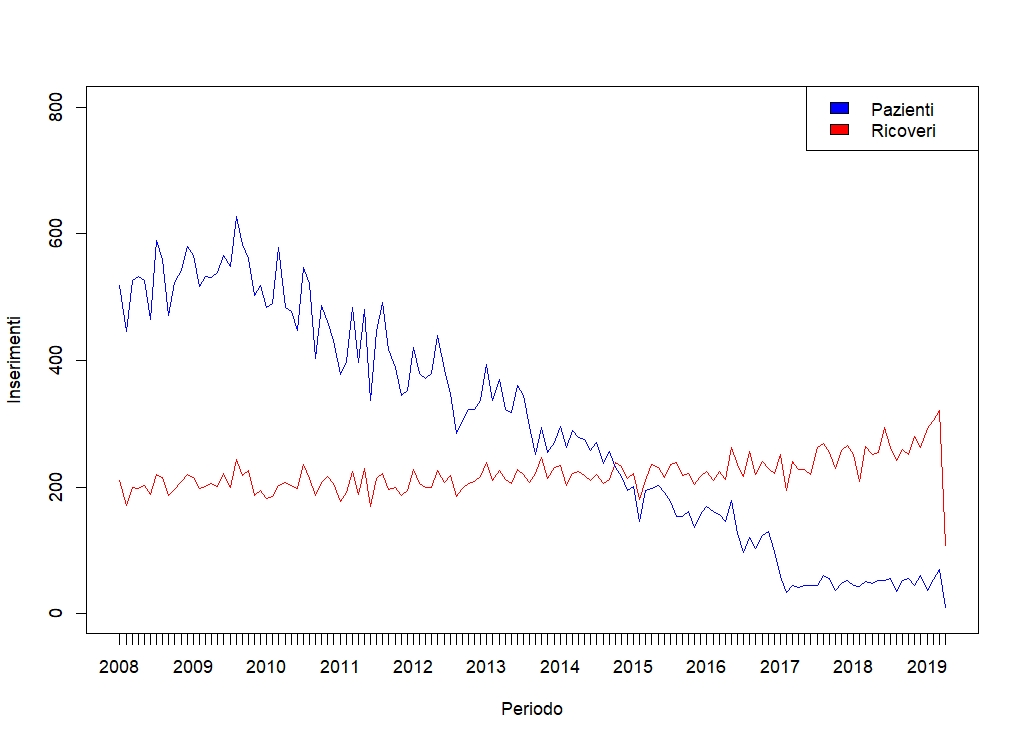
\includegraphics[width=\linewidth]{grafico_1}
  \caption{Andamento mensile inserimenti di Pazienti e di Ricoveri}
  \label{fig:grafico_1}
\end{figure}

Dal grafico si può intuire che
\begin{itemize}
  \item il numero di ricoveri inseriti mensilmente è soggetto ad una lenta crescita;
  \item il numero di nuove registrazioni, invece, sta calando notevolmente.
\end{itemize}
Se si mettono assieme le due informazioni si conclude che, in generale, un paziente che è già stato ricoverato almeno una volta, ha una probabilità maggiore, rispetto a qualche anno fa, di essere ricoverato nuovamente.

% TODO RIFARE GRAFICI TOGLIENDO ULTIMO MESE PERCHE INCOMPLETO
% Notare che i dati relativi all'ultimo mese nel grafico sono dati incompleti, poiché il mese deve ancora finire, quindi è perfettamente lecito che si trovino così in basso rispetto alla media.

\cleardoublepage


Richiesta: 
%In una media annuale, quante volte è stato ricoverato un paziente anziano(sopra i 60)? Ed uno giovane(sotto i 30)?
Annualmente quanti ricoveri riguardano un anziano (sopra i 60 anni)? Quanti riguardano un giovane (sotto i 30)?
\begin{figure}[!ht] % TODO abbellire
  \centering
  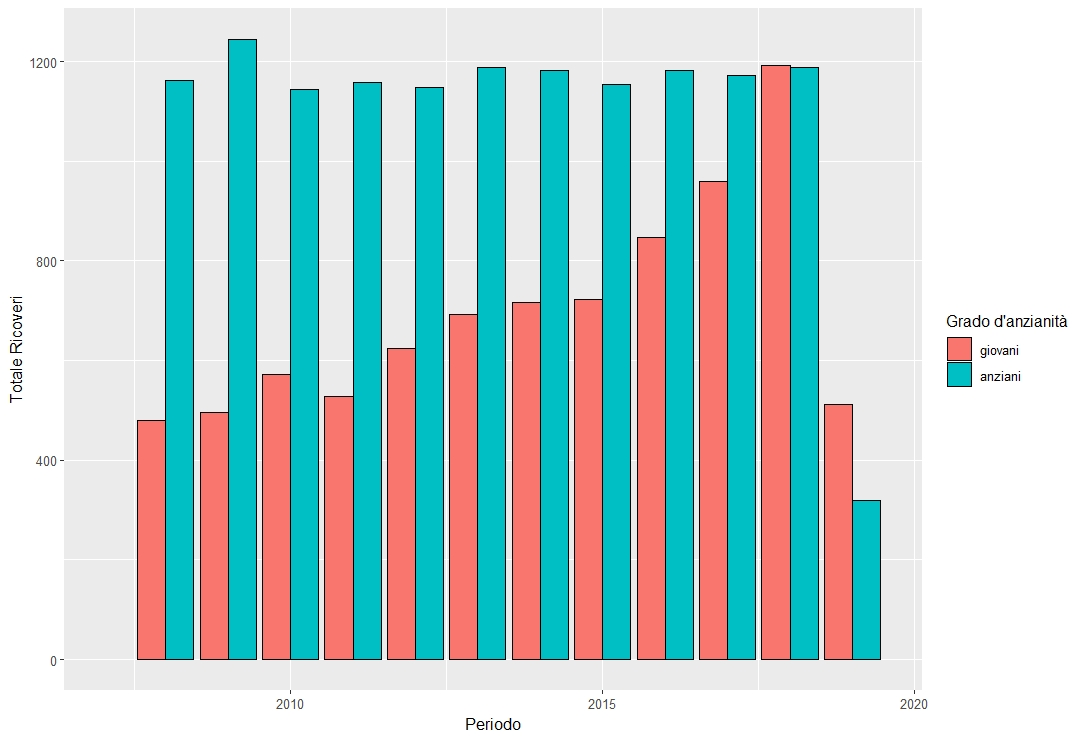
\includegraphics[width=\linewidth]{grafico_2}
  \caption{Ricoveri medi annui pazienti anziani vs giovani}
  \label{fig:grafico_2}
\end{figure}

Dal grafico si può notare che il numero di ricoveri di pazienti giovani è cresciuto notevolmente, mentre quello degli anziani è rimasto pressoché invariato.
Nel 2008 il numero di anziani ricoverati era oltre il doppio del numero di giovani, invece nel 2018 il numero di giovani, seppur di poco, ha addirittura superato il numero di anziani.
Questa tendenza potrebbe indicare che i giovani sono più cagionevoli di un tempo.
Con il prossimo grafico si vuole analizzare se la tendenza di cui sopra sia in qualche modo correlata alla crescente probabilità di sviluppare tumori in giovane età.

\cleardoublepage

Richiesta:
Annualmente a quanti giovani viene diagnosticato un tumore? A quanti anziani? A quanti nella fascia tra i 30 ed i 60 anni?
\begin{figure}[!ht] % TODO abbellire
  \centering
  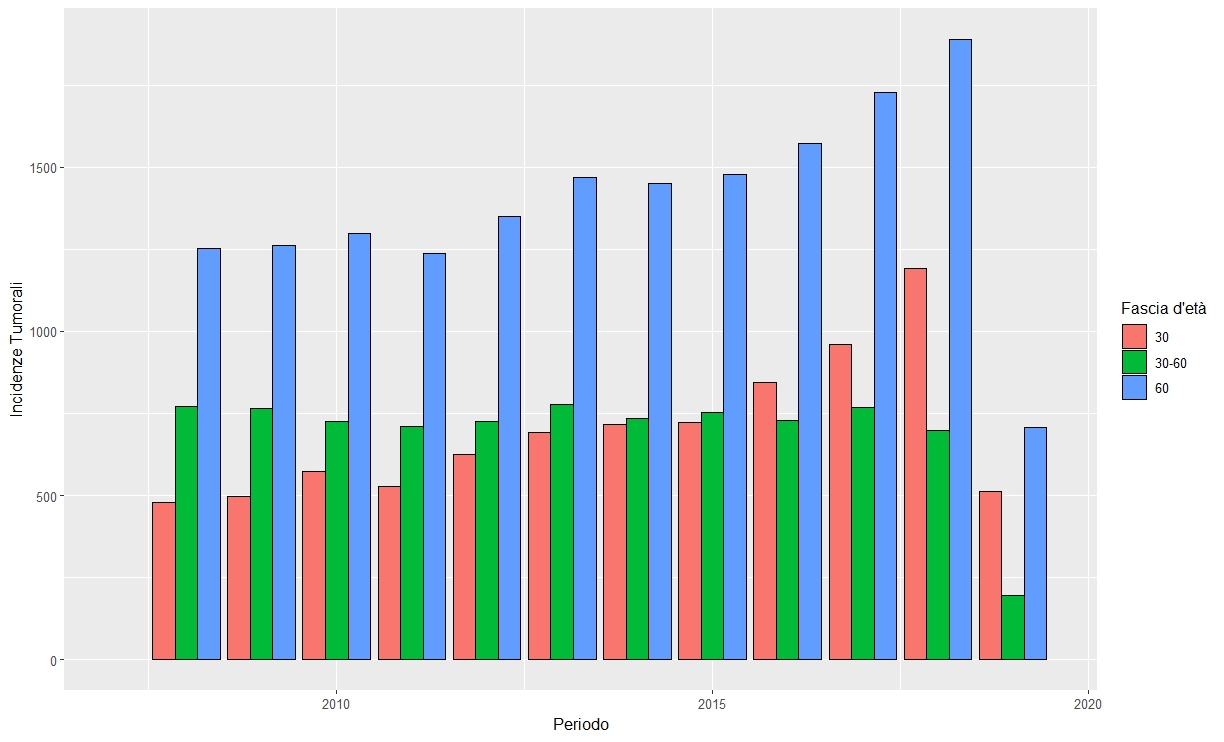
\includegraphics[width=\linewidth]{grafico_3}
  \caption{Ricoveri per tumore annui al variare delle età}
  \label{fig:grafico_3}
\end{figure}

Il grafico mostra chiaramente come i ricoveri per tumore sono sempre più frequenti per i giovani.
Anche la fascia d'età sopra i 60 segue un andamento simile.
Invece la fascia intermedia sembra avere una tendenza calante.
\cleardoublepage


Richiesta:
In quale periodo dell'anno ci sono più ricoveri per influenza? 
\begin{figure}[!ht] % TODO abbellire
  \centering
  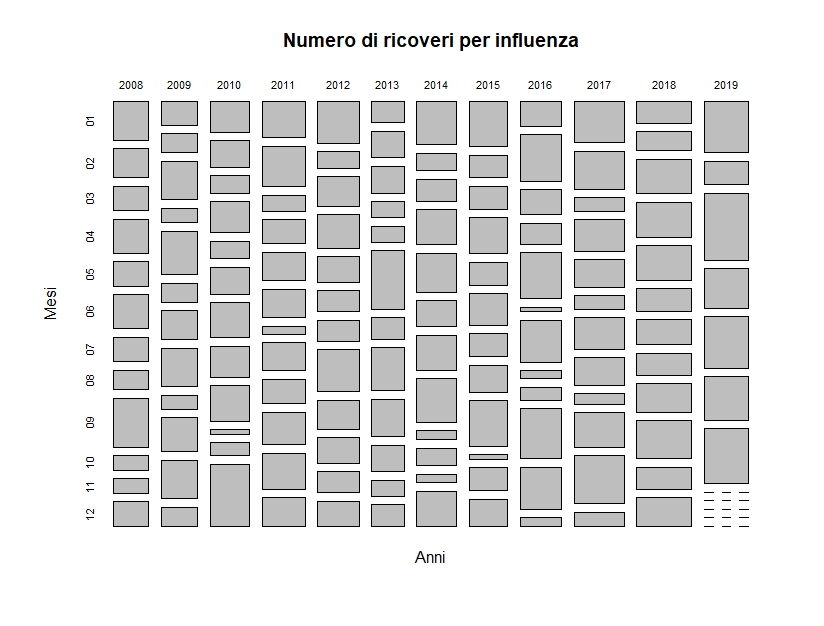
\includegraphics[width=.8\linewidth]{grafico_4}
  \caption{Ricoveri per influenza mensili al variare degli anni}
  \label{fig:grafico_4}

  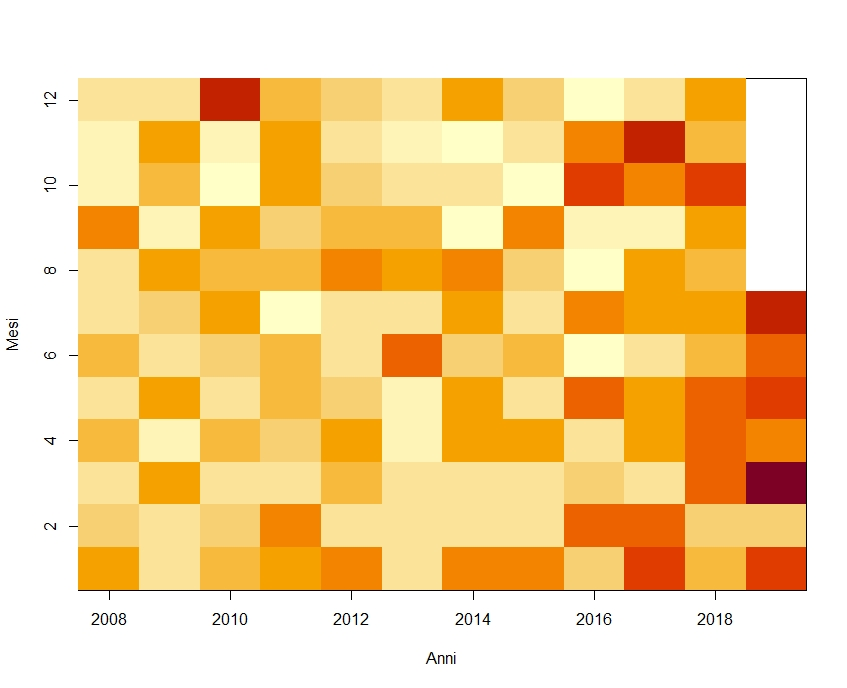
\includegraphics[width=.75\linewidth]{grafico_4-2}
  \caption{Ricoveri per influenza mensili al variare degli anni}
  \label{fig:grafico_4-2}
\end{figure}

% TODO dire in un italiano migliore
I due grafici rappresentano la stessa informazione.
Dal grafico a mosaico risulta più facile osservare l'andamento mensile di uno specifico anno, mentre il grafico \textit{heatmap} facilita il confronto di un mese al variare degli anni.
Ad esempio nel mese di dicembre del 2012 ci sono stati molti più ricoveri per influenza rispetto agli anni tra il 2014 ed il 2017.


\cleardoublepage


Richiesta:
Rispetto alle durate dei ricoveri in cui è stata diagnosticata una o più patologie tra le più frequenti, come si collocano le durate dei ricoveri legati a diagnosi per tumore?
 
\begin{figure}[!ht] % TODO abbellire
  \centering
  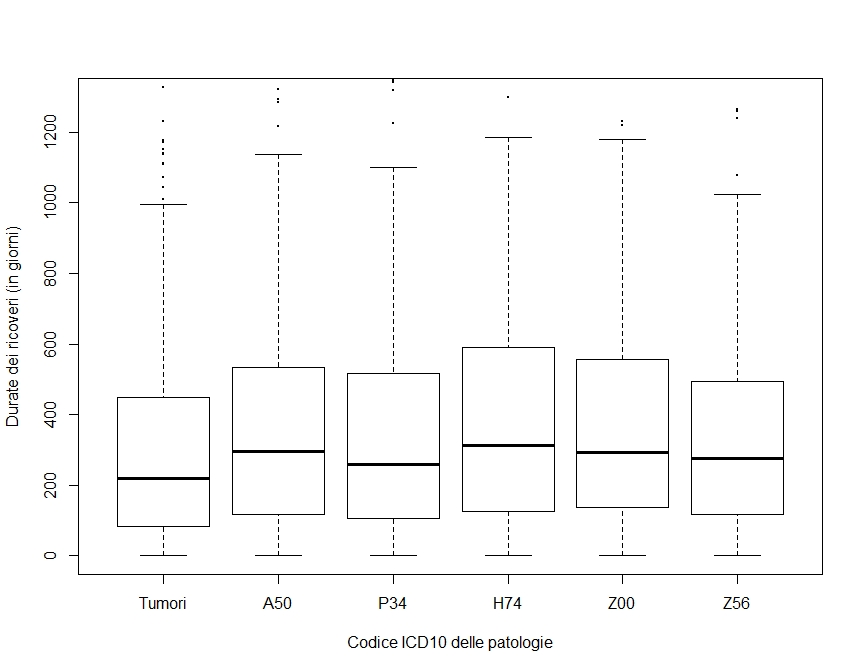
\includegraphics[width=\linewidth]{grafico_5}
  \caption{Confronto durate ricoveri per incidenze tumorali rispetto a quelli per patologie più frequenti}
  \label{fig:grafico_5}
\end{figure}

Il grafico mostra come la tendenza delle durate dei ricoveri per incidenze tumorali sia leggermente inferiore rispetto a quella dei ricoveri legati alle 5 patologie più frequenti. La distribuzione è asimmetrica in tutti i boxplot con una evidente variazione della distanza interquartilica rispetto alla mediana. 
Grazie a questa asimmetria è possibile notare come la durata dei ricoveri legati ai tumori sia leggermente meno variabile rispetto alle altre patologie considerate. In particolare, se la durata del ricovero supera i 200 giorni, potrebbe, statisticamente, proseguire per svariati giorni, in quanto un intervallo interquartilico maggiore implica una distribuzione più ampia. È interessante notare che alcuni valori anomali (outlier) indicano che per tutte le patologie considerate vi sono stati dei ricoveri che hanno avuto una durata di quasi 4 anni.

\cleardoublepage



\clearpage
\section{Progettazione Fisica}
\subsection{Nuovi Indici}
% Indice possibile è provincia 




\end{document}
